\documentclass[twoside]{book}

% Packages required by doxygen
\usepackage{fixltx2e}
\usepackage{calc}
\usepackage{doxygen}
\usepackage[export]{adjustbox} % also loads graphicx
\usepackage{graphicx}
\usepackage[utf8]{inputenc}
\usepackage{makeidx}
\usepackage{multicol}
\usepackage{multirow}
\PassOptionsToPackage{warn}{textcomp}
\usepackage{textcomp}
\usepackage[nointegrals]{wasysym}
\usepackage[table]{xcolor}

% Font selection
\usepackage[T1]{fontenc}
\usepackage[scaled=.90]{helvet}
\usepackage{courier}
\usepackage{amssymb}
\usepackage{sectsty}
\renewcommand{\familydefault}{\sfdefault}
\allsectionsfont{%
  \fontseries{bc}\selectfont%
  \color{darkgray}%
}
\renewcommand{\DoxyLabelFont}{%
  \fontseries{bc}\selectfont%
  \color{darkgray}%
}
\newcommand{\+}{\discretionary{\mbox{\scriptsize$\hookleftarrow$}}{}{}}

% Page & text layout
\usepackage{geometry}
\geometry{%
  a4paper,%
  top=2.5cm,%
  bottom=2.5cm,%
  left=2.5cm,%
  right=2.5cm%
}
\tolerance=750
\hfuzz=15pt
\hbadness=750
\setlength{\emergencystretch}{15pt}
\setlength{\parindent}{0cm}
\setlength{\parskip}{3ex plus 2ex minus 2ex}
\makeatletter
\renewcommand{\paragraph}{%
  \@startsection{paragraph}{4}{0ex}{-1.0ex}{1.0ex}{%
    \normalfont\normalsize\bfseries\SS@parafont%
  }%
}
\renewcommand{\subparagraph}{%
  \@startsection{subparagraph}{5}{0ex}{-1.0ex}{1.0ex}{%
    \normalfont\normalsize\bfseries\SS@subparafont%
  }%
}
\makeatother

% Headers & footers
\usepackage{fancyhdr}
\pagestyle{fancyplain}
\fancyhead[LE]{\fancyplain{}{\bfseries\thepage}}
\fancyhead[CE]{\fancyplain{}{}}
\fancyhead[RE]{\fancyplain{}{\bfseries\leftmark}}
\fancyhead[LO]{\fancyplain{}{\bfseries\rightmark}}
\fancyhead[CO]{\fancyplain{}{}}
\fancyhead[RO]{\fancyplain{}{\bfseries\thepage}}
\fancyfoot[LE]{\fancyplain{}{}}
\fancyfoot[CE]{\fancyplain{}{}}
\fancyfoot[RE]{\fancyplain{}{\bfseries\scriptsize Generated by Doxygen }}
\fancyfoot[LO]{\fancyplain{}{\bfseries\scriptsize Generated by Doxygen }}
\fancyfoot[CO]{\fancyplain{}{}}
\fancyfoot[RO]{\fancyplain{}{}}
\renewcommand{\footrulewidth}{0.4pt}
\renewcommand{\chaptermark}[1]{%
  \markboth{#1}{}%
}
\renewcommand{\sectionmark}[1]{%
  \markright{\thesection\ #1}%
}

% Indices & bibliography
\usepackage{natbib}
\usepackage[titles]{tocloft}
\setcounter{tocdepth}{3}
\setcounter{secnumdepth}{5}
\makeindex

% Custom commands
\newcommand{\clearemptydoublepage}{%
  \newpage{\pagestyle{empty}\cleardoublepage}%
}

\usepackage{caption}
\captionsetup{labelsep=space,justification=centering,font={bf},singlelinecheck=off,skip=4pt,position=top}

%===== C O N T E N T S =====

\begin{document}

% Titlepage & ToC
\pagenumbering{roman}
\begin{titlepage}
\vspace*{7cm}
\begin{center}%
{\Large Book Of Fame }\\
\vspace*{1cm}
{\large Generated by Doxygen 1.8.11}\\
\end{center}
\end{titlepage}
\clearemptydoublepage
\tableofcontents
\clearemptydoublepage
\pagenumbering{arabic}

%--- Begin generated contents ---
\chapter{Namespace Index}
\section{Packages}
Here are the packages with brief descriptions (if available)\+:\begin{DoxyCompactList}
\item\contentsline{section}{{\bf Assembly\+C\+Sharp} }{\pageref{namespace_assembly_c_sharp}}{}
\end{DoxyCompactList}

\chapter{Hierarchical Index}
\section{Class Hierarchy}
This inheritance list is sorted roughly, but not completely, alphabetically\+:\begin{DoxyCompactList}
\item \contentsline{section}{Annotation.\+Annotation\+Box}{\pageref{struct_annotation_1_1_annotation_box}}{}
\item \contentsline{section}{Assembly\+C\+Sharp.\+I\+I\+I\+F\+Get\+Manifest}{\pageref{class_assembly_c_sharp_1_1_i_i_i_f_get_manifest}}{}
\item Mono\+Behaviour\begin{DoxyCompactList}
\item \contentsline{section}{Annotation}{\pageref{class_annotation}}{}
\item \contentsline{section}{Annotation\+Drawer}{\pageref{class_annotation_drawer}}{}
\item \contentsline{section}{Annotation\+UI}{\pageref{class_annotation_u_i}}{}
\item \contentsline{section}{Book\+Handler}{\pageref{class_book_handler}}{}
\item \contentsline{section}{Button\+Controls}{\pageref{class_button_controls}}{}
\item \contentsline{section}{Camera\+Switch}{\pageref{class_camera_switch}}{}
\item \contentsline{section}{Dialog\+Box}{\pageref{class_dialog_box}}{}
\item \contentsline{section}{Hand\+On\+Page}{\pageref{class_hand_on_page}}{}
\item \contentsline{section}{I\+I\+I\+F\+Image\+Get}{\pageref{class_i_i_i_f_image_get}}{}
\item \contentsline{section}{I\+I\+I\+F\+Image\+Loading\+Bar}{\pageref{class_i_i_i_f_image_loading_bar}}{}
\item \contentsline{section}{Move}{\pageref{class_move}}{}
\item \contentsline{section}{Move\+Player}{\pageref{class_move_player}}{}
\item \contentsline{section}{Move\+Spotlight}{\pageref{class_move_spotlight}}{}
\item \contentsline{section}{Move\+Transcription\+Lens}{\pageref{class_move_transcription_lens}}{}
\item \contentsline{section}{Page\+Images}{\pageref{class_page_images}}{}
\item \contentsline{section}{Pop\+Up\+Box}{\pageref{class_pop_up_box}}{}
\item \contentsline{section}{Transcription\+Tool}{\pageref{class_transcription_tool}}{}
\item \contentsline{section}{U\+I\+Pop\+Up}{\pageref{class_u_i_pop_up}}{}
\end{DoxyCompactList}
\end{DoxyCompactList}

\chapter{Class Index}
\section{Class List}
Here are the classes, structs, unions and interfaces with brief descriptions\+:\begin{DoxyCompactList}
\item\contentsline{section}{{\bf Annotation} \\*Creates and retrieves annotations. }{\pageref{class_annotation}}{}
\item\contentsline{section}{{\bf Annotation.\+Annotation\+Box} \\*Contains data needed to display an annotation. }{\pageref{struct_annotation_1_1_annotation_box}}{}
\item\contentsline{section}{{\bf Annotation\+Drawer} \\*Draws annotation to the screen. }{\pageref{class_annotation_drawer}}{}
\item\contentsline{section}{{\bf Annotation\+UI} \\*Class that controls user interaction with individual annotations displayed on screen (currently does nothing, but may change in a future release). }{\pageref{class_annotation_u_i}}{}
\item\contentsline{section}{{\bf Book\+Handler} \\*Controls the opening and closing of the book. }{\pageref{class_book_handler}}{}
\item\contentsline{section}{{\bf Button\+Controls} \\*Stores infomation about the current tool. }{\pageref{class_button_controls}}{}
\item\contentsline{section}{{\bf Camera\+Switch} \\*Switches between the navigation and book mode cameras. }{\pageref{class_camera_switch}}{}
\item\contentsline{section}{{\bf Dialog\+Box} \\*A Dialog Box used to display text to the user. }{\pageref{class_dialog_box}}{}
\item\contentsline{section}{{\bf Hand\+On\+Page} \\*Controls page movement animation }{\pageref{class_hand_on_page}}{}
\item\contentsline{section}{{\bf Assembly\+C\+Sharp.\+I\+I\+I\+F\+Get\+Manifest} \\*Gets the manifest for a I\+I\+IF manuscript. }{\pageref{class_assembly_c_sharp_1_1_i_i_i_f_get_manifest}}{}
\item\contentsline{section}{{\bf I\+I\+I\+F\+Image\+Get} \\*Retrieves an image from an I\+I\+IF server. }{\pageref{class_i_i_i_f_image_get}}{}
\item\contentsline{section}{{\bf I\+I\+I\+F\+Image\+Loading\+Bar} \\*The loading bar for an I\+I\+IF image. }{\pageref{class_i_i_i_f_image_loading_bar}}{}
\item\contentsline{section}{{\bf Move} \\*The movement logic for the book mode camera. }{\pageref{class_move}}{}
\item\contentsline{section}{{\bf Move\+Player} \\*Movement logic for the navigation mode camera }{\pageref{class_move_player}}{}
\item\contentsline{section}{{\bf Move\+Spotlight} \\*The controls logic for the spotlight tool. }{\pageref{class_move_spotlight}}{}
\item\contentsline{section}{{\bf Move\+Transcription\+Lens} \\*The transcription lens movement logic. }{\pageref{class_move_transcription_lens}}{}
\item\contentsline{section}{{\bf Page\+Images} \\*Presents the I\+I\+IF images from a manifest on 6 pages. }{\pageref{class_page_images}}{}
\item\contentsline{section}{{\bf Pop\+Up\+Box} \\*A popup box used to get input from the user. }{\pageref{class_pop_up_box}}{}
\item\contentsline{section}{{\bf Transcription\+Tool} \\*Displays the transcription of the text. }{\pageref{class_transcription_tool}}{}
\item\contentsline{section}{{\bf U\+I\+Pop\+Up} \\*Hides/\+Shows UI elements. }{\pageref{class_u_i_pop_up}}{}
\end{DoxyCompactList}

\chapter{Namespace Documentation}
\section{Assembly\+C\+Sharp Namespace Reference}
\label{namespace_assembly_c_sharp}\index{Assembly\+C\+Sharp@{Assembly\+C\+Sharp}}
\subsection*{Classes}
\begin{DoxyCompactItemize}
\item 
class {\bf I\+I\+I\+F\+Get\+Manifest}
\begin{DoxyCompactList}\small\item\em Gets the manifest for a I\+I\+IF manuscript. \end{DoxyCompactList}\end{DoxyCompactItemize}

\chapter{Class Documentation}
\section{Annotation Class Reference}
\label{class_annotation}\index{Annotation@{Annotation}}


Creates and retrieves annotations.  


Inheritance diagram for Annotation\+:\begin{figure}[H]
\begin{center}
\leavevmode
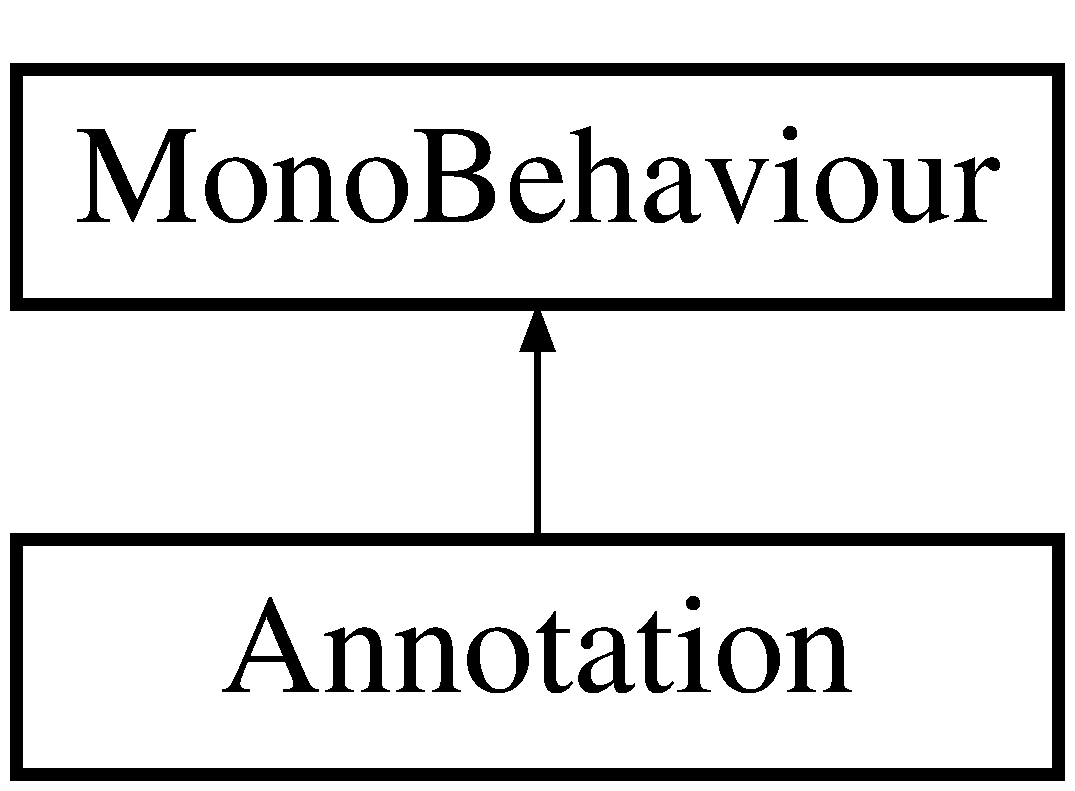
\includegraphics[height=2.000000cm]{class_annotation}
\end{center}
\end{figure}
\subsection*{Classes}
\begin{DoxyCompactItemize}
\item 
struct {\bf Annotation\+Box}
\begin{DoxyCompactList}\small\item\em Contains data needed to display an annotation. \end{DoxyCompactList}\end{DoxyCompactItemize}
\subsection*{Public Member Functions}
\begin{DoxyCompactItemize}
\item 
void {\bf Update\+Web\+Address} (string new\+Address)
\begin{DoxyCompactList}\small\item\em Updates the web address used for writting annotations. \end{DoxyCompactList}\item 
Array\+List {\bf Get\+Annotations} (string data, string url)
\begin{DoxyCompactList}\small\item\em Get all the annotations corresponding to a specific I\+I\+IF image. \end{DoxyCompactList}\item 
string {\bf Local\+Annotation\+File} ()
\begin{DoxyCompactList}\small\item\em Get the path to the local annotation file. \end{DoxyCompactList}\end{DoxyCompactItemize}
\subsection*{Public Attributes}
\begin{DoxyCompactItemize}
\item 
int {\bf page\+Width}
\begin{DoxyCompactList}\small\item\em The width of the image. \end{DoxyCompactList}\item 
int {\bf page\+Height}
\begin{DoxyCompactList}\small\item\em The height of the image. \end{DoxyCompactList}\item 
Collider {\bf page}
\begin{DoxyCompactList}\small\item\em The Collider used to calculate where on the page the user clicked. \end{DoxyCompactList}\item 
{\bf Page\+Images} {\bfseries webdata}\label{class_annotation_a349cea2640123c51730779a08eaaf8e1}

\item 
Transform {\bf top\+Left}
\begin{DoxyCompactList}\small\item\em The location of the top left corner of the page. \end{DoxyCompactList}\item 
Transform {\bf bottom\+Right}
\begin{DoxyCompactList}\small\item\em The location of the bottom right corner of the page. \end{DoxyCompactList}\item 
string {\bf web\+Address}
\begin{DoxyCompactList}\small\item\em The web address to write to the annotation file. \end{DoxyCompactList}\end{DoxyCompactItemize}


\subsection{Detailed Description}
Creates and retrieves annotations. 



\subsection{Member Function Documentation}
\index{Annotation@{Annotation}!Get\+Annotations@{Get\+Annotations}}
\index{Get\+Annotations@{Get\+Annotations}!Annotation@{Annotation}}
\subsubsection[{Get\+Annotations(string data, string url)}]{\setlength{\rightskip}{0pt plus 5cm}Array\+List Annotation.\+Get\+Annotations (
\begin{DoxyParamCaption}
\item[{string}]{data, }
\item[{string}]{url}
\end{DoxyParamCaption}
)}\label{class_annotation_a6f51b2747ec2eae72f61bd83fd9d47a7}


Get all the annotations corresponding to a specific I\+I\+IF image. 

\begin{DoxyReturn}{Returns}
An Array\+List of all the annotations corresponding to a webpage (each annotation is an \doxyref{Annotation\+Box}{p.}{struct_annotation_1_1_annotation_box}).
\end{DoxyReturn}

\begin{DoxyParams}{Parameters}
{\em data} & The source annotation file to parse as a String.\\
\hline
{\em url} & The U\+RL that represents the I\+I\+IF image to look for annotations for.\\
\hline
\end{DoxyParams}
\index{Annotation@{Annotation}!Local\+Annotation\+File@{Local\+Annotation\+File}}
\index{Local\+Annotation\+File@{Local\+Annotation\+File}!Annotation@{Annotation}}
\subsubsection[{Local\+Annotation\+File()}]{\setlength{\rightskip}{0pt plus 5cm}string Annotation.\+Local\+Annotation\+File (
\begin{DoxyParamCaption}
{}
\end{DoxyParamCaption}
)}\label{class_annotation_ad60e0259e6a6a490d7e2e250e7a121a6}


Get the path to the local annotation file. 

\begin{DoxyReturn}{Returns}
The path to the local annotation file.
\end{DoxyReturn}
\index{Annotation@{Annotation}!Update\+Web\+Address@{Update\+Web\+Address}}
\index{Update\+Web\+Address@{Update\+Web\+Address}!Annotation@{Annotation}}
\subsubsection[{Update\+Web\+Address(string new\+Address)}]{\setlength{\rightskip}{0pt plus 5cm}void Annotation.\+Update\+Web\+Address (
\begin{DoxyParamCaption}
\item[{string}]{new\+Address}
\end{DoxyParamCaption}
)}\label{class_annotation_aec2adf7ea1bf592d75c43133df56d33d}


Updates the web address used for writting annotations. 


\begin{DoxyParams}{Parameters}
{\em new\+Address} & The new web address to write for new annotations.\\
\hline
\end{DoxyParams}


\subsection{Member Data Documentation}
\index{Annotation@{Annotation}!bottom\+Right@{bottom\+Right}}
\index{bottom\+Right@{bottom\+Right}!Annotation@{Annotation}}
\subsubsection[{bottom\+Right}]{\setlength{\rightskip}{0pt plus 5cm}Transform Annotation.\+bottom\+Right}\label{class_annotation_a784e68c2876b721c7332ad8c4d19d4b4}


The location of the bottom right corner of the page. 

\index{Annotation@{Annotation}!page@{page}}
\index{page@{page}!Annotation@{Annotation}}
\subsubsection[{page}]{\setlength{\rightskip}{0pt plus 5cm}Collider Annotation.\+page}\label{class_annotation_a89356eeb4c128231a7542016d61fe35c}


The Collider used to calculate where on the page the user clicked. 

\index{Annotation@{Annotation}!page\+Height@{page\+Height}}
\index{page\+Height@{page\+Height}!Annotation@{Annotation}}
\subsubsection[{page\+Height}]{\setlength{\rightskip}{0pt plus 5cm}int Annotation.\+page\+Height}\label{class_annotation_a6ed1263c99626c3db9c3af44d7853761}


The height of the image. 

The height used to calculate annotation coordinates \index{Annotation@{Annotation}!page\+Width@{page\+Width}}
\index{page\+Width@{page\+Width}!Annotation@{Annotation}}
\subsubsection[{page\+Width}]{\setlength{\rightskip}{0pt plus 5cm}int Annotation.\+page\+Width}\label{class_annotation_a3eeea869dfc405c3ed8b3556cf4181b7}


The width of the image. 

The width used to calculate annotation coordinates \index{Annotation@{Annotation}!top\+Left@{top\+Left}}
\index{top\+Left@{top\+Left}!Annotation@{Annotation}}
\subsubsection[{top\+Left}]{\setlength{\rightskip}{0pt plus 5cm}Transform Annotation.\+top\+Left}\label{class_annotation_a6701449aed12538b4be40a9d2f1a9898}


The location of the top left corner of the page. 

\index{Annotation@{Annotation}!web\+Address@{web\+Address}}
\index{web\+Address@{web\+Address}!Annotation@{Annotation}}
\subsubsection[{web\+Address}]{\setlength{\rightskip}{0pt plus 5cm}string Annotation.\+web\+Address}\label{class_annotation_adb6d8fefb4974f1ff1d0f0a031455f37}


The web address to write to the annotation file. 



The documentation for this class was generated from the following file\+:\begin{DoxyCompactItemize}
\item 
Annotation.\+cs\end{DoxyCompactItemize}

\section{Annotation.\+Annotation\+Box Struct Reference}
\label{struct_annotation_1_1_annotation_box}\index{Annotation.\+Annotation\+Box@{Annotation.\+Annotation\+Box}}


Contains data needed to display an annotation.  


\subsection*{Public Attributes}
\begin{DoxyCompactItemize}
\item 
string {\bf contents}
\begin{DoxyCompactList}\small\item\em The contents of the annotation. \end{DoxyCompactList}\item 
float {\bf x}
\begin{DoxyCompactList}\small\item\em The horizontal offset of the annotation from the left side of the page, as a percentage of page width. \end{DoxyCompactList}\item 
float {\bf y}
\begin{DoxyCompactList}\small\item\em The vertical offset of the annotation from the top side of the page, as a percentage of page height. \end{DoxyCompactList}\item 
float {\bf w}
\begin{DoxyCompactList}\small\item\em The width of the annotation, as a percentage of page width. \end{DoxyCompactList}\item 
float {\bf h}
\begin{DoxyCompactList}\small\item\em The height of the annotation, as a percentage of page height. \end{DoxyCompactList}\end{DoxyCompactItemize}


\subsection{Detailed Description}
Contains data needed to display an annotation. 



\subsection{Member Data Documentation}
\index{Annotation\+::\+Annotation\+Box@{Annotation\+::\+Annotation\+Box}!contents@{contents}}
\index{contents@{contents}!Annotation\+::\+Annotation\+Box@{Annotation\+::\+Annotation\+Box}}
\subsubsection[{contents}]{\setlength{\rightskip}{0pt plus 5cm}string Annotation.\+Annotation\+Box.\+contents}\label{struct_annotation_1_1_annotation_box_a34dbf8361a6e99dec24a2e34f2235a47}


The contents of the annotation. 

\index{Annotation\+::\+Annotation\+Box@{Annotation\+::\+Annotation\+Box}!h@{h}}
\index{h@{h}!Annotation\+::\+Annotation\+Box@{Annotation\+::\+Annotation\+Box}}
\subsubsection[{h}]{\setlength{\rightskip}{0pt plus 5cm}float Annotation.\+Annotation\+Box.\+h}\label{struct_annotation_1_1_annotation_box_ae1b9fc84cb44650938afc0622f2a73d7}


The height of the annotation, as a percentage of page height. 

\index{Annotation\+::\+Annotation\+Box@{Annotation\+::\+Annotation\+Box}!w@{w}}
\index{w@{w}!Annotation\+::\+Annotation\+Box@{Annotation\+::\+Annotation\+Box}}
\subsubsection[{w}]{\setlength{\rightskip}{0pt plus 5cm}float Annotation.\+Annotation\+Box.\+w}\label{struct_annotation_1_1_annotation_box_a8351fba84fd574b466abdc8922444524}


The width of the annotation, as a percentage of page width. 

\index{Annotation\+::\+Annotation\+Box@{Annotation\+::\+Annotation\+Box}!x@{x}}
\index{x@{x}!Annotation\+::\+Annotation\+Box@{Annotation\+::\+Annotation\+Box}}
\subsubsection[{x}]{\setlength{\rightskip}{0pt plus 5cm}float Annotation.\+Annotation\+Box.\+x}\label{struct_annotation_1_1_annotation_box_a6e431b3be4693eec2a05836305c951b7}


The horizontal offset of the annotation from the left side of the page, as a percentage of page width. 

\index{Annotation\+::\+Annotation\+Box@{Annotation\+::\+Annotation\+Box}!y@{y}}
\index{y@{y}!Annotation\+::\+Annotation\+Box@{Annotation\+::\+Annotation\+Box}}
\subsubsection[{y}]{\setlength{\rightskip}{0pt plus 5cm}float Annotation.\+Annotation\+Box.\+y}\label{struct_annotation_1_1_annotation_box_abe016787ca879c554211b47dfc6b7965}


The vertical offset of the annotation from the top side of the page, as a percentage of page height. 



The documentation for this struct was generated from the following file\+:\begin{DoxyCompactItemize}
\item 
Annotation.\+cs\end{DoxyCompactItemize}

\section{Annotation\+Drawer Class Reference}
\label{class_annotation_drawer}\index{Annotation\+Drawer@{Annotation\+Drawer}}


Draws annotation to the screen.  


Inheritance diagram for Annotation\+Drawer\+:\begin{figure}[H]
\begin{center}
\leavevmode
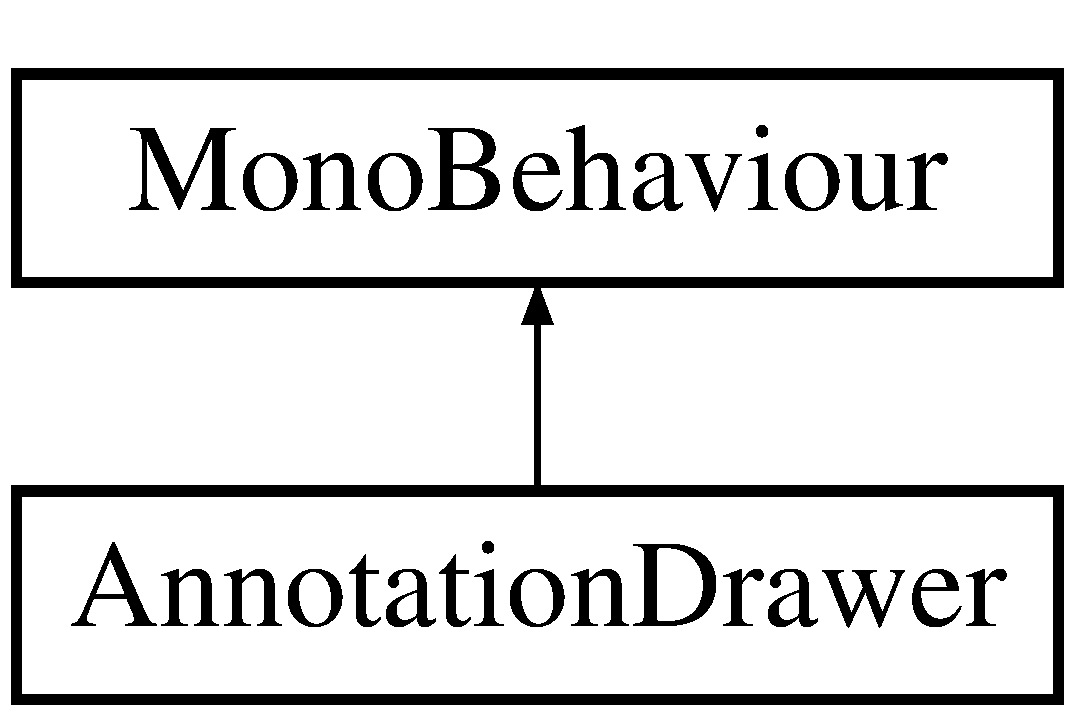
\includegraphics[height=2.000000cm]{class_annotation_drawer}
\end{center}
\end{figure}
\subsection*{Public Member Functions}
\begin{DoxyCompactItemize}
\item 
void {\bf Updates\+Annotations} ({\bf Annotation.\+Annotation\+Box}[$\,$] annos)
\begin{DoxyCompactList}\small\item\em Updates the annotations this instance draws. \end{DoxyCompactList}\item 
void {\bf Show\+Annotations} (bool is\+Showing)
\begin{DoxyCompactList}\small\item\em Shows/\+Hides the annotations. \end{DoxyCompactList}\end{DoxyCompactItemize}
\subsection*{Public Attributes}
\begin{DoxyCompactItemize}
\item 
Transform {\bf top\+Left}
\begin{DoxyCompactList}\small\item\em The top left corner of the page to draw to. \end{DoxyCompactList}\item 
Transform {\bf bottom\+Right}
\begin{DoxyCompactList}\small\item\em The bottom right corner of the page to draw to. \end{DoxyCompactList}\item 
Transform {\bf anno\+Obj}
\begin{DoxyCompactList}\small\item\em The annotation object to draw. \end{DoxyCompactList}\item 
Transform {\bf canvas}
\begin{DoxyCompactList}\small\item\em The location of the canvas. \end{DoxyCompactList}\end{DoxyCompactItemize}


\subsection{Detailed Description}
Draws annotation to the screen. 



\subsection{Member Function Documentation}
\index{Annotation\+Drawer@{Annotation\+Drawer}!Show\+Annotations@{Show\+Annotations}}
\index{Show\+Annotations@{Show\+Annotations}!Annotation\+Drawer@{Annotation\+Drawer}}
\subsubsection[{Show\+Annotations(bool is\+Showing)}]{\setlength{\rightskip}{0pt plus 5cm}void Annotation\+Drawer.\+Show\+Annotations (
\begin{DoxyParamCaption}
\item[{bool}]{is\+Showing}
\end{DoxyParamCaption}
)}\label{class_annotation_drawer_ac123d95b60addde272d0b946dba7ba75}


Shows/\+Hides the annotations. 


\begin{DoxyParams}{Parameters}
{\em is\+Showing} & If set to {\ttfamily true} show the annotations, else hides the annotations.\\
\hline
\end{DoxyParams}
\index{Annotation\+Drawer@{Annotation\+Drawer}!Updates\+Annotations@{Updates\+Annotations}}
\index{Updates\+Annotations@{Updates\+Annotations}!Annotation\+Drawer@{Annotation\+Drawer}}
\subsubsection[{Updates\+Annotations(\+Annotation.\+Annotation\+Box[] annos)}]{\setlength{\rightskip}{0pt plus 5cm}void Annotation\+Drawer.\+Updates\+Annotations (
\begin{DoxyParamCaption}
\item[{{\bf Annotation.\+Annotation\+Box}[$\,$]}]{annos}
\end{DoxyParamCaption}
)}\label{class_annotation_drawer_a58b5001b2b927121bd9faf0036105590}


Updates the annotations this instance draws. 


\begin{DoxyParams}{Parameters}
{\em annos} & The new annotations to draw.\\
\hline
\end{DoxyParams}


\subsection{Member Data Documentation}
\index{Annotation\+Drawer@{Annotation\+Drawer}!anno\+Obj@{anno\+Obj}}
\index{anno\+Obj@{anno\+Obj}!Annotation\+Drawer@{Annotation\+Drawer}}
\subsubsection[{anno\+Obj}]{\setlength{\rightskip}{0pt plus 5cm}Transform Annotation\+Drawer.\+anno\+Obj}\label{class_annotation_drawer_a65eb569e2f2251ae40599541cac14a81}


The annotation object to draw. 

\index{Annotation\+Drawer@{Annotation\+Drawer}!bottom\+Right@{bottom\+Right}}
\index{bottom\+Right@{bottom\+Right}!Annotation\+Drawer@{Annotation\+Drawer}}
\subsubsection[{bottom\+Right}]{\setlength{\rightskip}{0pt plus 5cm}Transform Annotation\+Drawer.\+bottom\+Right}\label{class_annotation_drawer_a5cedf015a42cc5bef94c956344217e88}


The bottom right corner of the page to draw to. 

\index{Annotation\+Drawer@{Annotation\+Drawer}!canvas@{canvas}}
\index{canvas@{canvas}!Annotation\+Drawer@{Annotation\+Drawer}}
\subsubsection[{canvas}]{\setlength{\rightskip}{0pt plus 5cm}Transform Annotation\+Drawer.\+canvas}\label{class_annotation_drawer_a82fe9da03536f06847e78186e0c175a1}


The location of the canvas. 

\index{Annotation\+Drawer@{Annotation\+Drawer}!top\+Left@{top\+Left}}
\index{top\+Left@{top\+Left}!Annotation\+Drawer@{Annotation\+Drawer}}
\subsubsection[{top\+Left}]{\setlength{\rightskip}{0pt plus 5cm}Transform Annotation\+Drawer.\+top\+Left}\label{class_annotation_drawer_a932f3cf8744289386ec6950d41638f30}


The top left corner of the page to draw to. 



The documentation for this class was generated from the following file\+:\begin{DoxyCompactItemize}
\item 
Annotation\+Drawer.\+cs\end{DoxyCompactItemize}

\section{Annotation\+UI Class Reference}
\label{class_annotation_u_i}\index{Annotation\+UI@{Annotation\+UI}}


Class that controls user interaction with individual annotations displayed on screen (currently does nothing, but may change in a future release).  


Inheritance diagram for Annotation\+UI\+:\begin{figure}[H]
\begin{center}
\leavevmode
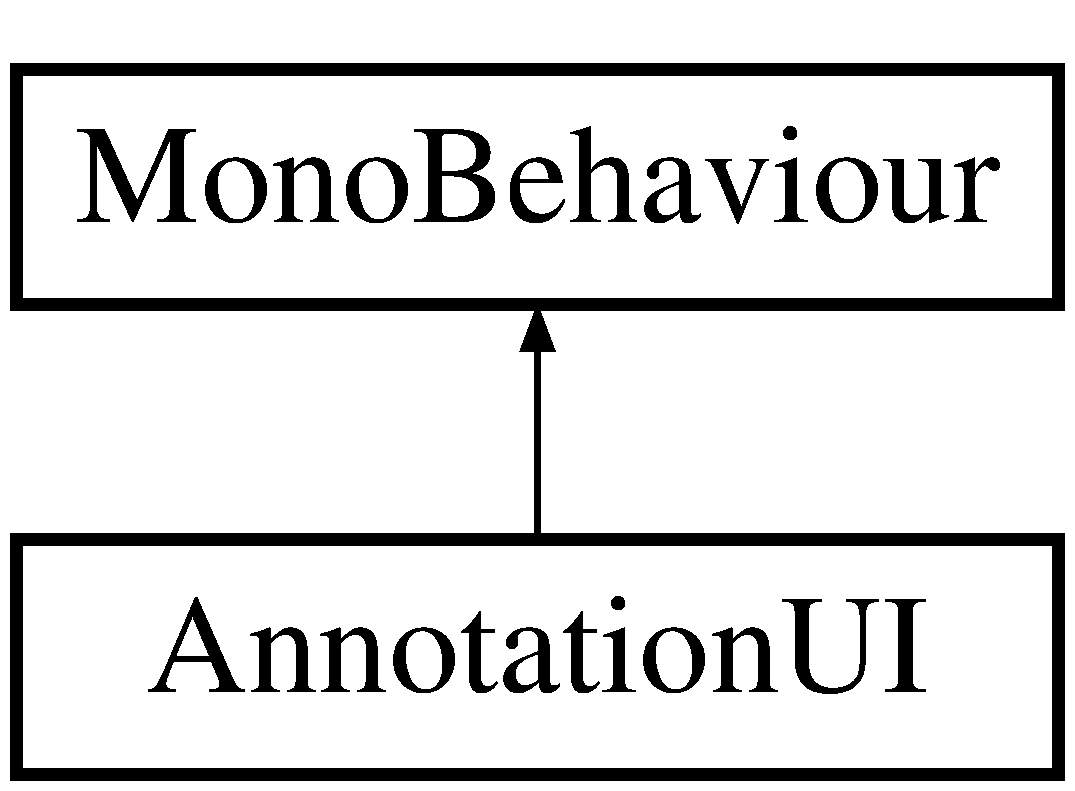
\includegraphics[height=2.000000cm]{class_annotation_u_i}
\end{center}
\end{figure}


\subsection{Detailed Description}
Class that controls user interaction with individual annotations displayed on screen (currently does nothing, but may change in a future release). 



The documentation for this class was generated from the following file\+:\begin{DoxyCompactItemize}
\item 
Annotation\+U\+I.\+cs\end{DoxyCompactItemize}

\section{Book\+Handler Class Reference}
\label{class_book_handler}\index{Book\+Handler@{Book\+Handler}}


Controls the opening and closing of the book.  


Inheritance diagram for Book\+Handler\+:\begin{figure}[H]
\begin{center}
\leavevmode
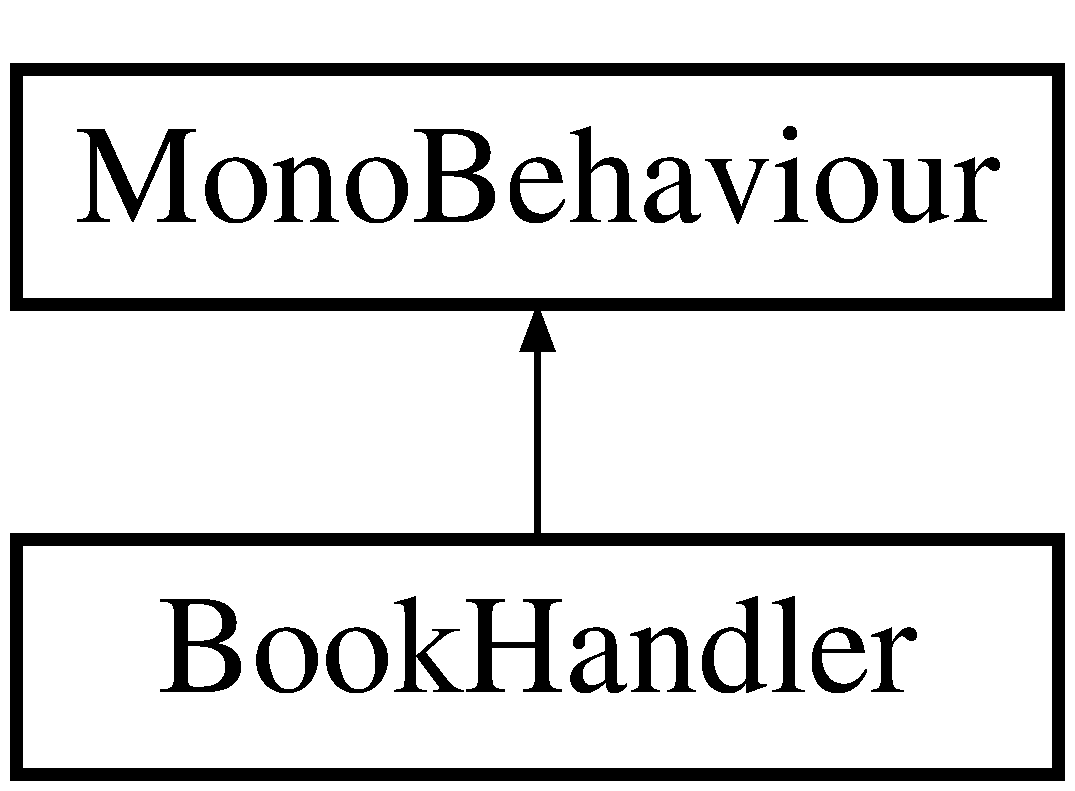
\includegraphics[height=2.000000cm]{class_book_handler}
\end{center}
\end{figure}
\subsection*{Public Attributes}
\begin{DoxyCompactItemize}
\item 
Animator {\bf animator}
\begin{DoxyCompactList}\small\item\em The animator of the book. \end{DoxyCompactList}\item 
Game\+Object {\bf pages}
\begin{DoxyCompactList}\small\item\em The pages of the book. \end{DoxyCompactList}\item 
Collider[$\,$] {\bf models}
\begin{DoxyCompactList}\small\item\em The Colliders for the front and back covers of the book. \end{DoxyCompactList}\item 
{\bf U\+I\+Pop\+Up} {\bf my\+UI}
\begin{DoxyCompactList}\small\item\em The Toolbar UI. \end{DoxyCompactList}\end{DoxyCompactItemize}


\subsection{Detailed Description}
Controls the opening and closing of the book. 



\subsection{Member Data Documentation}
\index{Book\+Handler@{Book\+Handler}!animator@{animator}}
\index{animator@{animator}!Book\+Handler@{Book\+Handler}}
\subsubsection[{animator}]{\setlength{\rightskip}{0pt plus 5cm}Animator Book\+Handler.\+animator}\label{class_book_handler_aee55e4d0b6978567f3b9fe7ced515631}


The animator of the book. 

\index{Book\+Handler@{Book\+Handler}!models@{models}}
\index{models@{models}!Book\+Handler@{Book\+Handler}}
\subsubsection[{models}]{\setlength{\rightskip}{0pt plus 5cm}Collider [$\,$] Book\+Handler.\+models}\label{class_book_handler_a3e0579bd892b63ba3fad5b7284df1774}


The Colliders for the front and back covers of the book. 

\index{Book\+Handler@{Book\+Handler}!my\+UI@{my\+UI}}
\index{my\+UI@{my\+UI}!Book\+Handler@{Book\+Handler}}
\subsubsection[{my\+UI}]{\setlength{\rightskip}{0pt plus 5cm}{\bf U\+I\+Pop\+Up} Book\+Handler.\+my\+UI}\label{class_book_handler_aafcf17dc285ab162e349fe84b1ba119b}


The Toolbar UI. 

\index{Book\+Handler@{Book\+Handler}!pages@{pages}}
\index{pages@{pages}!Book\+Handler@{Book\+Handler}}
\subsubsection[{pages}]{\setlength{\rightskip}{0pt plus 5cm}Game\+Object Book\+Handler.\+pages}\label{class_book_handler_ac559d4edb6409bd60793a9e94e02f67a}


The pages of the book. 



The documentation for this class was generated from the following file\+:\begin{DoxyCompactItemize}
\item 
Book\+Handler.\+cs\end{DoxyCompactItemize}

\section{Button\+Controls Class Reference}
\label{class_button_controls}\index{Button\+Controls@{Button\+Controls}}


Stores infomation about the current tool.  


Inheritance diagram for Button\+Controls\+:\begin{figure}[H]
\begin{center}
\leavevmode
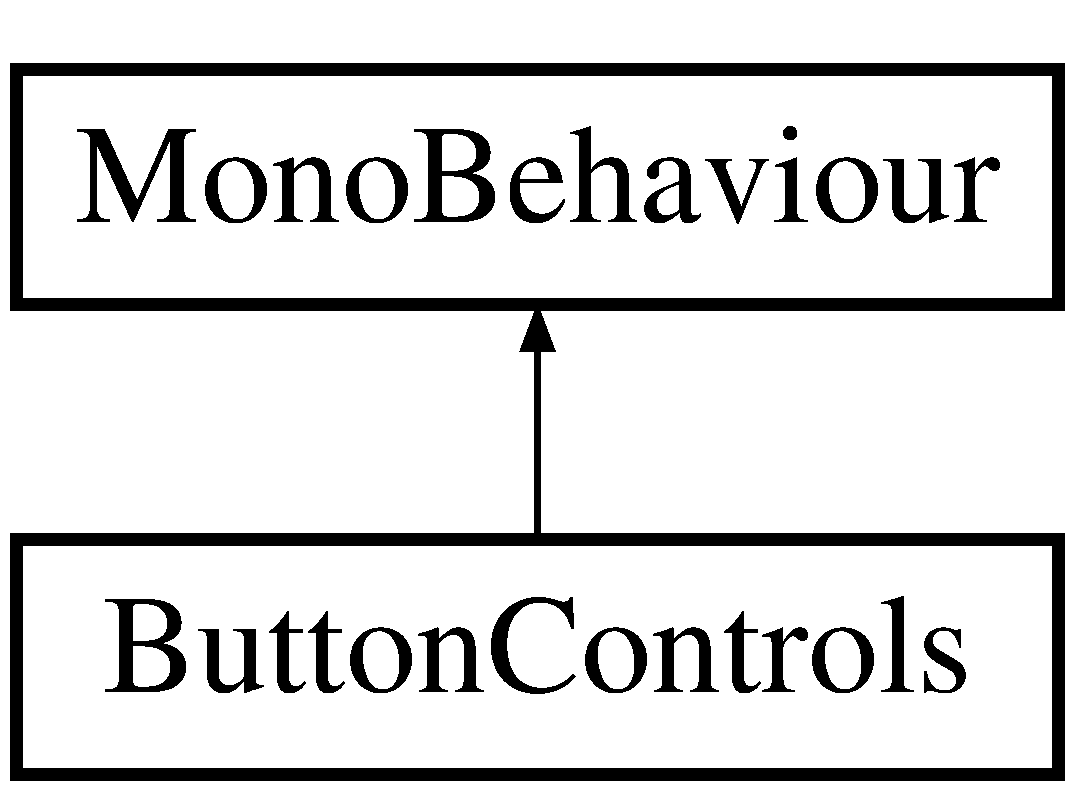
\includegraphics[height=2.000000cm]{class_button_controls}
\end{center}
\end{figure}
\subsection*{Public Member Functions}
\begin{DoxyCompactItemize}
\item 
I\+Enumerator {\bf Pop\+Up} ()
\begin{DoxyCompactList}\small\item\em Causes a popup window to be display, prompting the user for input. \end{DoxyCompactList}\item 
string {\bf get\+Popup\+Text} ()
\begin{DoxyCompactList}\small\item\em Gets the text from the popup window. \end{DoxyCompactList}\item 
int {\bf get\+Selected} ()
\begin{DoxyCompactList}\small\item\em Gets the currently selected tool. \end{DoxyCompactList}\item 
void {\bf change\+Selected} (int new\+Selected)
\begin{DoxyCompactList}\small\item\em Changes the currently selected tool. \end{DoxyCompactList}\item 
void {\bf clear\+Selected} ()
\begin{DoxyCompactList}\small\item\em Makes no tool be selected. \end{DoxyCompactList}\item 
void {\bf Show\+Latest\+Tweet} ()
\begin{DoxyCompactList}\small\item\em Shows the latest tweet from our twitter account. \end{DoxyCompactList}\item 
I\+Enumerator {\bf Hide\+Tweet\+Box} ()
\begin{DoxyCompactList}\small\item\em Hides the tweet box. \end{DoxyCompactList}\end{DoxyCompactItemize}
\subsection*{Public Attributes}
\begin{DoxyCompactItemize}
\item 
Button[$\,$] {\bf buttons}
\begin{DoxyCompactList}\small\item\em The buttons for the tools. \end{DoxyCompactList}\item 
Image[$\,$] {\bf images}
\begin{DoxyCompactList}\small\item\em The images for the tools. \end{DoxyCompactList}\item 
{\bf Pop\+Up\+Box} {\bf popup}
\begin{DoxyCompactList}\small\item\em The Popup window to use to get text input from the user. \end{DoxyCompactList}\item 
{\bf Move} {\bf book\+Cam}
\begin{DoxyCompactList}\small\item\em The camera for book mode \end{DoxyCompactList}\item 
{\bf Camera\+Switch} {\bf switcher}
\begin{DoxyCompactList}\small\item\em The switcher between navigation mode and book mode cameras. \end{DoxyCompactList}\item 
{\bf Page\+Images} {\bf presenter}
\begin{DoxyCompactList}\small\item\em The presenter of the I\+I\+IF images. \end{DoxyCompactList}\item 
Game\+Object {\bf tweet\+Box}
\begin{DoxyCompactList}\small\item\em The box used to display tweets. \end{DoxyCompactList}\item 
Text {\bf tweet\+Text}
\begin{DoxyCompactList}\small\item\em The text in the tweet\+Box containing the text of the tweet. \end{DoxyCompactList}\item 
bool {\bf is\+Spotlight} = false
\begin{DoxyCompactList}\small\item\em Is the spotlight on? \end{DoxyCompactList}\item 
{\bf Move\+Spotlight} {\bf spotlight}
\begin{DoxyCompactList}\small\item\em The spotlight. \end{DoxyCompactList}\item 
Game\+Object {\bf twitter\+Bird\+Obj}
\begin{DoxyCompactList}\small\item\em The twitter bird. \end{DoxyCompactList}\item 
Image {\bf twitter\+Bird}
\begin{DoxyCompactList}\small\item\em The twitter bird\textquotesingle{}s image. \end{DoxyCompactList}\item 
Sprite {\bf twitter\+Bird\+Closed}
\begin{DoxyCompactList}\small\item\em The twitter bird\textquotesingle{}s idle image. \end{DoxyCompactList}\item 
Sprite {\bf twitter\+Bird\+Open}
\begin{DoxyCompactList}\small\item\em The twitter bird\textquotesingle{}s talking image. \end{DoxyCompactList}\item 
Audio\+Source {\bf twitter\+Sound}
\begin{DoxyCompactList}\small\item\em The sound to play when the twitter bird is talking. \end{DoxyCompactList}\item 
{\bf Dialog\+Box} {\bf dialog}
\begin{DoxyCompactList}\small\item\em The dialog box to use to display text to the user. \end{DoxyCompactList}\item 
const int {\bf L\+I\+G\+H\+T\+\_\+\+T\+O\+OL} = 0
\begin{DoxyCompactList}\small\item\em The ID for the Light Tool. \end{DoxyCompactList}\item 
const int {\bf A\+N\+N\+O\+T\+A\+T\+I\+O\+N\+\_\+\+T\+O\+OL} = 1
\begin{DoxyCompactList}\small\item\em The ID for the \doxyref{Annotation}{p.}{class_annotation} Tool. \end{DoxyCompactList}\item 
const int {\bf H\+A\+N\+D\+\_\+\+T\+O\+OL} = 2
\begin{DoxyCompactList}\small\item\em The ID for the Hand Tool. \end{DoxyCompactList}\item 
const int {\bf D\+I\+R\+E\+C\+T\+O\+R\+Y\+\_\+\+T\+O\+OL} = 3
\begin{DoxyCompactList}\small\item\em The ID for the Directory Tool. \end{DoxyCompactList}\item 
const int {\bf R\+E\+A\+D\+E\+R\+\_\+\+T\+O\+OL} = 4
\begin{DoxyCompactList}\small\item\em The ID for the Display Annotations Tool. \end{DoxyCompactList}\item 
const int {\bf S\+E\+L\+E\+C\+T\+I\+O\+N\+\_\+\+T\+O\+OL} = 6
\begin{DoxyCompactList}\small\item\em The ID for the Open/\+Close Book Tool. \end{DoxyCompactList}\item 
const int {\bf Z\+O\+O\+M\+\_\+\+T\+O\+OL} = 5
\begin{DoxyCompactList}\small\item\em The ID for the Zoom Tool (currently not used). \end{DoxyCompactList}\item 
const int {\bf L\+E\+N\+S\+\_\+\+T\+O\+OL} = 8
\begin{DoxyCompactList}\small\item\em The ID for the Transcription Tool. \end{DoxyCompactList}\item 
const int {\bf T\+W\+I\+T\+T\+E\+R\+\_\+\+T\+O\+OL} = 9
\begin{DoxyCompactList}\small\item\em The ID for the Twitter Tool. \end{DoxyCompactList}\end{DoxyCompactItemize}
\subsection*{Static Public Attributes}
\begin{DoxyCompactItemize}
\item 
static {\bf Button\+Controls} {\bf current}
\begin{DoxyCompactList}\small\item\em The current \doxyref{Button\+Controls}{p.}{class_button_controls} instance. \end{DoxyCompactList}\end{DoxyCompactItemize}


\subsection{Detailed Description}
Stores infomation about the current tool. 



\subsection{Member Function Documentation}
\index{Button\+Controls@{Button\+Controls}!change\+Selected@{change\+Selected}}
\index{change\+Selected@{change\+Selected}!Button\+Controls@{Button\+Controls}}
\subsubsection[{change\+Selected(int new\+Selected)}]{\setlength{\rightskip}{0pt plus 5cm}void Button\+Controls.\+change\+Selected (
\begin{DoxyParamCaption}
\item[{int}]{new\+Selected}
\end{DoxyParamCaption}
)}\label{class_button_controls_a5b0bee37e9fd14beb3d5ab43afe6213c}


Changes the currently selected tool. 


\begin{DoxyParams}{Parameters}
{\em new\+Selected} & The tool to select.\\
\hline
\end{DoxyParams}
\index{Button\+Controls@{Button\+Controls}!clear\+Selected@{clear\+Selected}}
\index{clear\+Selected@{clear\+Selected}!Button\+Controls@{Button\+Controls}}
\subsubsection[{clear\+Selected()}]{\setlength{\rightskip}{0pt plus 5cm}void Button\+Controls.\+clear\+Selected (
\begin{DoxyParamCaption}
{}
\end{DoxyParamCaption}
)}\label{class_button_controls_a0850e47668086c4311eb6edcc40ecc8a}


Makes no tool be selected. 

\index{Button\+Controls@{Button\+Controls}!get\+Popup\+Text@{get\+Popup\+Text}}
\index{get\+Popup\+Text@{get\+Popup\+Text}!Button\+Controls@{Button\+Controls}}
\subsubsection[{get\+Popup\+Text()}]{\setlength{\rightskip}{0pt plus 5cm}string Button\+Controls.\+get\+Popup\+Text (
\begin{DoxyParamCaption}
{}
\end{DoxyParamCaption}
)}\label{class_button_controls_af54ecb5ed2899a6a9302431f8df94833}


Gets the text from the popup window. 

\begin{DoxyReturn}{Returns}
The text inputed into the popup window.
\end{DoxyReturn}
\index{Button\+Controls@{Button\+Controls}!get\+Selected@{get\+Selected}}
\index{get\+Selected@{get\+Selected}!Button\+Controls@{Button\+Controls}}
\subsubsection[{get\+Selected()}]{\setlength{\rightskip}{0pt plus 5cm}int Button\+Controls.\+get\+Selected (
\begin{DoxyParamCaption}
{}
\end{DoxyParamCaption}
)}\label{class_button_controls_a1610d1a14723fdf450ded1e8818ce425}


Gets the currently selected tool. 

\begin{DoxyReturn}{Returns}
The integer id of the currently selected tool.
\end{DoxyReturn}
\index{Button\+Controls@{Button\+Controls}!Hide\+Tweet\+Box@{Hide\+Tweet\+Box}}
\index{Hide\+Tweet\+Box@{Hide\+Tweet\+Box}!Button\+Controls@{Button\+Controls}}
\subsubsection[{Hide\+Tweet\+Box()}]{\setlength{\rightskip}{0pt plus 5cm}I\+Enumerator Button\+Controls.\+Hide\+Tweet\+Box (
\begin{DoxyParamCaption}
{}
\end{DoxyParamCaption}
)}\label{class_button_controls_a5f598b3dda96d7e9c50e00730e744482}


Hides the tweet box. 

\index{Button\+Controls@{Button\+Controls}!Pop\+Up@{Pop\+Up}}
\index{Pop\+Up@{Pop\+Up}!Button\+Controls@{Button\+Controls}}
\subsubsection[{Pop\+Up()}]{\setlength{\rightskip}{0pt plus 5cm}I\+Enumerator Button\+Controls.\+Pop\+Up (
\begin{DoxyParamCaption}
{}
\end{DoxyParamCaption}
)}\label{class_button_controls_a02c9477eba81f169ed58199b6aac5f34}


Causes a popup window to be display, prompting the user for input. 

\index{Button\+Controls@{Button\+Controls}!Show\+Latest\+Tweet@{Show\+Latest\+Tweet}}
\index{Show\+Latest\+Tweet@{Show\+Latest\+Tweet}!Button\+Controls@{Button\+Controls}}
\subsubsection[{Show\+Latest\+Tweet()}]{\setlength{\rightskip}{0pt plus 5cm}void Button\+Controls.\+Show\+Latest\+Tweet (
\begin{DoxyParamCaption}
{}
\end{DoxyParamCaption}
)}\label{class_button_controls_a3a2f044c63295b78c205415070768e38}


Shows the latest tweet from our twitter account. 



\subsection{Member Data Documentation}
\index{Button\+Controls@{Button\+Controls}!A\+N\+N\+O\+T\+A\+T\+I\+O\+N\+\_\+\+T\+O\+OL@{A\+N\+N\+O\+T\+A\+T\+I\+O\+N\+\_\+\+T\+O\+OL}}
\index{A\+N\+N\+O\+T\+A\+T\+I\+O\+N\+\_\+\+T\+O\+OL@{A\+N\+N\+O\+T\+A\+T\+I\+O\+N\+\_\+\+T\+O\+OL}!Button\+Controls@{Button\+Controls}}
\subsubsection[{A\+N\+N\+O\+T\+A\+T\+I\+O\+N\+\_\+\+T\+O\+OL}]{\setlength{\rightskip}{0pt plus 5cm}const int Button\+Controls.\+A\+N\+N\+O\+T\+A\+T\+I\+O\+N\+\_\+\+T\+O\+OL = 1}\label{class_button_controls_a5b464828976bb242314a92890e0a0818}


The ID for the \doxyref{Annotation}{p.}{class_annotation} Tool. 

\index{Button\+Controls@{Button\+Controls}!book\+Cam@{book\+Cam}}
\index{book\+Cam@{book\+Cam}!Button\+Controls@{Button\+Controls}}
\subsubsection[{book\+Cam}]{\setlength{\rightskip}{0pt plus 5cm}{\bf Move} Button\+Controls.\+book\+Cam}\label{class_button_controls_a01ede77b80cc6e1b032a20710384e2be}


The camera for book mode 

\index{Button\+Controls@{Button\+Controls}!buttons@{buttons}}
\index{buttons@{buttons}!Button\+Controls@{Button\+Controls}}
\subsubsection[{buttons}]{\setlength{\rightskip}{0pt plus 5cm}Button [$\,$] Button\+Controls.\+buttons}\label{class_button_controls_a6d8481d8d10b1764500df5ebff2754c3}


The buttons for the tools. 

\index{Button\+Controls@{Button\+Controls}!current@{current}}
\index{current@{current}!Button\+Controls@{Button\+Controls}}
\subsubsection[{current}]{\setlength{\rightskip}{0pt plus 5cm}{\bf Button\+Controls} Button\+Controls.\+current\hspace{0.3cm}{\ttfamily [static]}}\label{class_button_controls_a8104ade53ad756b5a0c70f282b614aa1}


The current \doxyref{Button\+Controls}{p.}{class_button_controls} instance. 

\index{Button\+Controls@{Button\+Controls}!dialog@{dialog}}
\index{dialog@{dialog}!Button\+Controls@{Button\+Controls}}
\subsubsection[{dialog}]{\setlength{\rightskip}{0pt plus 5cm}{\bf Dialog\+Box} Button\+Controls.\+dialog}\label{class_button_controls_ad0ce254085aa49db69c0a1422849cc84}


The dialog box to use to display text to the user. 

\index{Button\+Controls@{Button\+Controls}!D\+I\+R\+E\+C\+T\+O\+R\+Y\+\_\+\+T\+O\+OL@{D\+I\+R\+E\+C\+T\+O\+R\+Y\+\_\+\+T\+O\+OL}}
\index{D\+I\+R\+E\+C\+T\+O\+R\+Y\+\_\+\+T\+O\+OL@{D\+I\+R\+E\+C\+T\+O\+R\+Y\+\_\+\+T\+O\+OL}!Button\+Controls@{Button\+Controls}}
\subsubsection[{D\+I\+R\+E\+C\+T\+O\+R\+Y\+\_\+\+T\+O\+OL}]{\setlength{\rightskip}{0pt plus 5cm}const int Button\+Controls.\+D\+I\+R\+E\+C\+T\+O\+R\+Y\+\_\+\+T\+O\+OL = 3}\label{class_button_controls_af863f78b5d287a50df76c65a31942ef7}


The ID for the Directory Tool. 

\index{Button\+Controls@{Button\+Controls}!H\+A\+N\+D\+\_\+\+T\+O\+OL@{H\+A\+N\+D\+\_\+\+T\+O\+OL}}
\index{H\+A\+N\+D\+\_\+\+T\+O\+OL@{H\+A\+N\+D\+\_\+\+T\+O\+OL}!Button\+Controls@{Button\+Controls}}
\subsubsection[{H\+A\+N\+D\+\_\+\+T\+O\+OL}]{\setlength{\rightskip}{0pt plus 5cm}const int Button\+Controls.\+H\+A\+N\+D\+\_\+\+T\+O\+OL = 2}\label{class_button_controls_af773f1e77c187f3b4f4200b54ed94ca3}


The ID for the Hand Tool. 

\index{Button\+Controls@{Button\+Controls}!images@{images}}
\index{images@{images}!Button\+Controls@{Button\+Controls}}
\subsubsection[{images}]{\setlength{\rightskip}{0pt plus 5cm}Image [$\,$] Button\+Controls.\+images}\label{class_button_controls_a4e95044b881d63cd2a1e593467ee0287}


The images for the tools. 

\index{Button\+Controls@{Button\+Controls}!is\+Spotlight@{is\+Spotlight}}
\index{is\+Spotlight@{is\+Spotlight}!Button\+Controls@{Button\+Controls}}
\subsubsection[{is\+Spotlight}]{\setlength{\rightskip}{0pt plus 5cm}bool Button\+Controls.\+is\+Spotlight = false}\label{class_button_controls_ae537b21797d71dc696c80cba3e2ba061}


Is the spotlight on? 

\index{Button\+Controls@{Button\+Controls}!L\+E\+N\+S\+\_\+\+T\+O\+OL@{L\+E\+N\+S\+\_\+\+T\+O\+OL}}
\index{L\+E\+N\+S\+\_\+\+T\+O\+OL@{L\+E\+N\+S\+\_\+\+T\+O\+OL}!Button\+Controls@{Button\+Controls}}
\subsubsection[{L\+E\+N\+S\+\_\+\+T\+O\+OL}]{\setlength{\rightskip}{0pt plus 5cm}const int Button\+Controls.\+L\+E\+N\+S\+\_\+\+T\+O\+OL = 8}\label{class_button_controls_a0832c77868b3b2084d282bdd06309fd7}


The ID for the Transcription Tool. 

\index{Button\+Controls@{Button\+Controls}!L\+I\+G\+H\+T\+\_\+\+T\+O\+OL@{L\+I\+G\+H\+T\+\_\+\+T\+O\+OL}}
\index{L\+I\+G\+H\+T\+\_\+\+T\+O\+OL@{L\+I\+G\+H\+T\+\_\+\+T\+O\+OL}!Button\+Controls@{Button\+Controls}}
\subsubsection[{L\+I\+G\+H\+T\+\_\+\+T\+O\+OL}]{\setlength{\rightskip}{0pt plus 5cm}const int Button\+Controls.\+L\+I\+G\+H\+T\+\_\+\+T\+O\+OL = 0}\label{class_button_controls_a12957783dbbfb938853778c29c9f0d60}


The ID for the Light Tool. 

\index{Button\+Controls@{Button\+Controls}!popup@{popup}}
\index{popup@{popup}!Button\+Controls@{Button\+Controls}}
\subsubsection[{popup}]{\setlength{\rightskip}{0pt plus 5cm}{\bf Pop\+Up\+Box} Button\+Controls.\+popup}\label{class_button_controls_a01a5f62a3985cbea7f08821c39beaa39}


The Popup window to use to get text input from the user. 

\index{Button\+Controls@{Button\+Controls}!presenter@{presenter}}
\index{presenter@{presenter}!Button\+Controls@{Button\+Controls}}
\subsubsection[{presenter}]{\setlength{\rightskip}{0pt plus 5cm}{\bf Page\+Images} Button\+Controls.\+presenter}\label{class_button_controls_a37e94945a8c9614569aa2b089f449609}


The presenter of the I\+I\+IF images. 

\index{Button\+Controls@{Button\+Controls}!R\+E\+A\+D\+E\+R\+\_\+\+T\+O\+OL@{R\+E\+A\+D\+E\+R\+\_\+\+T\+O\+OL}}
\index{R\+E\+A\+D\+E\+R\+\_\+\+T\+O\+OL@{R\+E\+A\+D\+E\+R\+\_\+\+T\+O\+OL}!Button\+Controls@{Button\+Controls}}
\subsubsection[{R\+E\+A\+D\+E\+R\+\_\+\+T\+O\+OL}]{\setlength{\rightskip}{0pt plus 5cm}const int Button\+Controls.\+R\+E\+A\+D\+E\+R\+\_\+\+T\+O\+OL = 4}\label{class_button_controls_a45bd648b6f9269a063939e3e5ce487a0}


The ID for the Display Annotations Tool. 

\index{Button\+Controls@{Button\+Controls}!S\+E\+L\+E\+C\+T\+I\+O\+N\+\_\+\+T\+O\+OL@{S\+E\+L\+E\+C\+T\+I\+O\+N\+\_\+\+T\+O\+OL}}
\index{S\+E\+L\+E\+C\+T\+I\+O\+N\+\_\+\+T\+O\+OL@{S\+E\+L\+E\+C\+T\+I\+O\+N\+\_\+\+T\+O\+OL}!Button\+Controls@{Button\+Controls}}
\subsubsection[{S\+E\+L\+E\+C\+T\+I\+O\+N\+\_\+\+T\+O\+OL}]{\setlength{\rightskip}{0pt plus 5cm}const int Button\+Controls.\+S\+E\+L\+E\+C\+T\+I\+O\+N\+\_\+\+T\+O\+OL = 6}\label{class_button_controls_acfa8075ce363581c665d643e1cd2a1f5}


The ID for the Open/\+Close Book Tool. 

\index{Button\+Controls@{Button\+Controls}!spotlight@{spotlight}}
\index{spotlight@{spotlight}!Button\+Controls@{Button\+Controls}}
\subsubsection[{spotlight}]{\setlength{\rightskip}{0pt plus 5cm}{\bf Move\+Spotlight} Button\+Controls.\+spotlight}\label{class_button_controls_aaf795798730a8acb3765b1f8c03e5e7b}


The spotlight. 

\index{Button\+Controls@{Button\+Controls}!switcher@{switcher}}
\index{switcher@{switcher}!Button\+Controls@{Button\+Controls}}
\subsubsection[{switcher}]{\setlength{\rightskip}{0pt plus 5cm}{\bf Camera\+Switch} Button\+Controls.\+switcher}\label{class_button_controls_a8f473bdad9552060fe27ecd37ad5e573}


The switcher between navigation mode and book mode cameras. 

\index{Button\+Controls@{Button\+Controls}!tweet\+Box@{tweet\+Box}}
\index{tweet\+Box@{tweet\+Box}!Button\+Controls@{Button\+Controls}}
\subsubsection[{tweet\+Box}]{\setlength{\rightskip}{0pt plus 5cm}Game\+Object Button\+Controls.\+tweet\+Box}\label{class_button_controls_afa3096e052a7483a01d74dd25ce55941}


The box used to display tweets. 

\index{Button\+Controls@{Button\+Controls}!tweet\+Text@{tweet\+Text}}
\index{tweet\+Text@{tweet\+Text}!Button\+Controls@{Button\+Controls}}
\subsubsection[{tweet\+Text}]{\setlength{\rightskip}{0pt plus 5cm}Text Button\+Controls.\+tweet\+Text}\label{class_button_controls_aa18893c5233e5fb021f9ca7dddd22c3b}


The text in the tweet\+Box containing the text of the tweet. 

\index{Button\+Controls@{Button\+Controls}!T\+W\+I\+T\+T\+E\+R\+\_\+\+T\+O\+OL@{T\+W\+I\+T\+T\+E\+R\+\_\+\+T\+O\+OL}}
\index{T\+W\+I\+T\+T\+E\+R\+\_\+\+T\+O\+OL@{T\+W\+I\+T\+T\+E\+R\+\_\+\+T\+O\+OL}!Button\+Controls@{Button\+Controls}}
\subsubsection[{T\+W\+I\+T\+T\+E\+R\+\_\+\+T\+O\+OL}]{\setlength{\rightskip}{0pt plus 5cm}const int Button\+Controls.\+T\+W\+I\+T\+T\+E\+R\+\_\+\+T\+O\+OL = 9}\label{class_button_controls_a7c37ceab26948e379ed703daab8b4046}


The ID for the Twitter Tool. 

\index{Button\+Controls@{Button\+Controls}!twitter\+Bird@{twitter\+Bird}}
\index{twitter\+Bird@{twitter\+Bird}!Button\+Controls@{Button\+Controls}}
\subsubsection[{twitter\+Bird}]{\setlength{\rightskip}{0pt plus 5cm}Image Button\+Controls.\+twitter\+Bird}\label{class_button_controls_ad1a93855fb9dfc7f93f2ba635558a8eb}


The twitter bird\textquotesingle{}s image. 

\index{Button\+Controls@{Button\+Controls}!twitter\+Bird\+Closed@{twitter\+Bird\+Closed}}
\index{twitter\+Bird\+Closed@{twitter\+Bird\+Closed}!Button\+Controls@{Button\+Controls}}
\subsubsection[{twitter\+Bird\+Closed}]{\setlength{\rightskip}{0pt plus 5cm}Sprite Button\+Controls.\+twitter\+Bird\+Closed}\label{class_button_controls_af5b7db66d7e12459215994f28cf8b10d}


The twitter bird\textquotesingle{}s idle image. 

\index{Button\+Controls@{Button\+Controls}!twitter\+Bird\+Obj@{twitter\+Bird\+Obj}}
\index{twitter\+Bird\+Obj@{twitter\+Bird\+Obj}!Button\+Controls@{Button\+Controls}}
\subsubsection[{twitter\+Bird\+Obj}]{\setlength{\rightskip}{0pt plus 5cm}Game\+Object Button\+Controls.\+twitter\+Bird\+Obj}\label{class_button_controls_ac765e8ce56a53ab49931b21bc5d20083}


The twitter bird. 

\index{Button\+Controls@{Button\+Controls}!twitter\+Bird\+Open@{twitter\+Bird\+Open}}
\index{twitter\+Bird\+Open@{twitter\+Bird\+Open}!Button\+Controls@{Button\+Controls}}
\subsubsection[{twitter\+Bird\+Open}]{\setlength{\rightskip}{0pt plus 5cm}Sprite Button\+Controls.\+twitter\+Bird\+Open}\label{class_button_controls_a51f7c83d58220a5f8ecb5ffbb31c9eb7}


The twitter bird\textquotesingle{}s talking image. 

\index{Button\+Controls@{Button\+Controls}!twitter\+Sound@{twitter\+Sound}}
\index{twitter\+Sound@{twitter\+Sound}!Button\+Controls@{Button\+Controls}}
\subsubsection[{twitter\+Sound}]{\setlength{\rightskip}{0pt plus 5cm}Audio\+Source Button\+Controls.\+twitter\+Sound}\label{class_button_controls_aca201bf52f1b0290d3c69e450f1978fb}


The sound to play when the twitter bird is talking. 

\index{Button\+Controls@{Button\+Controls}!Z\+O\+O\+M\+\_\+\+T\+O\+OL@{Z\+O\+O\+M\+\_\+\+T\+O\+OL}}
\index{Z\+O\+O\+M\+\_\+\+T\+O\+OL@{Z\+O\+O\+M\+\_\+\+T\+O\+OL}!Button\+Controls@{Button\+Controls}}
\subsubsection[{Z\+O\+O\+M\+\_\+\+T\+O\+OL}]{\setlength{\rightskip}{0pt plus 5cm}const int Button\+Controls.\+Z\+O\+O\+M\+\_\+\+T\+O\+OL = 5}\label{class_button_controls_a4c4a3cb66d3bca032986166a818ae28e}


The ID for the Zoom Tool (currently not used). 



The documentation for this class was generated from the following file\+:\begin{DoxyCompactItemize}
\item 
Button\+Controls.\+cs\end{DoxyCompactItemize}

\section{Camera\+Switch Class Reference}
\label{class_camera_switch}\index{Camera\+Switch@{Camera\+Switch}}


Switches between the navigation and book mode cameras.  


Inheritance diagram for Camera\+Switch\+:\begin{figure}[H]
\begin{center}
\leavevmode
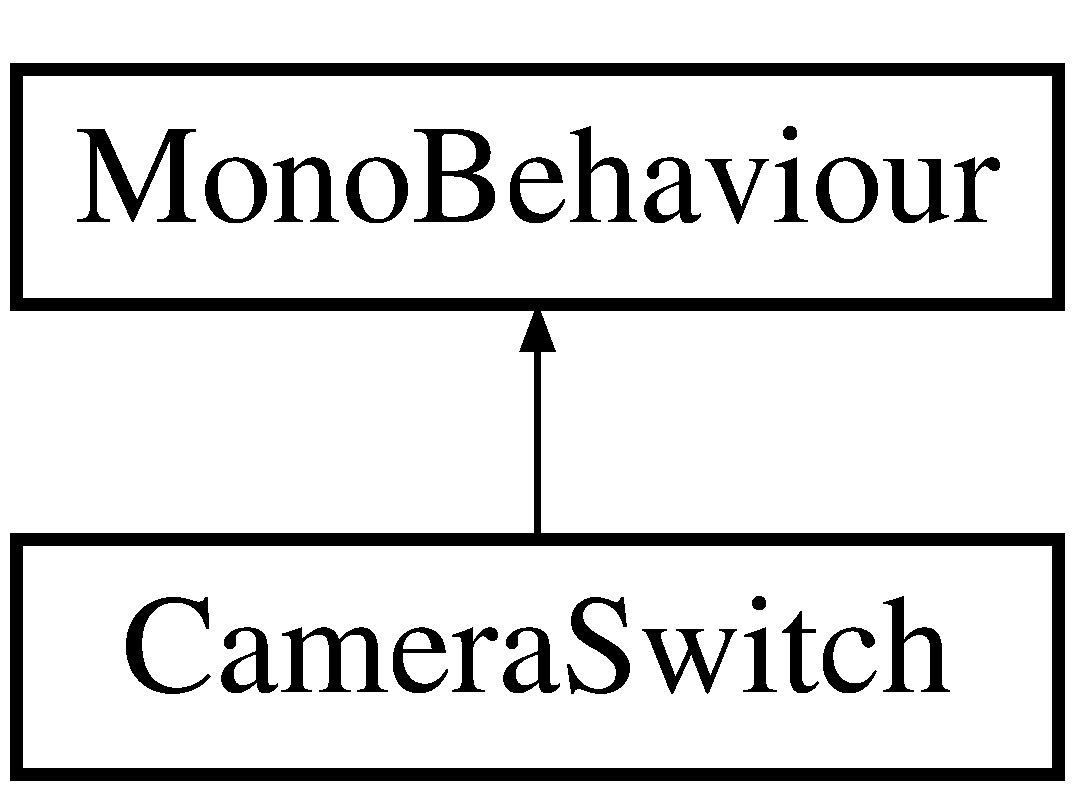
\includegraphics[height=2.000000cm]{class_camera_switch}
\end{center}
\end{figure}
\subsection*{Public Attributes}
\begin{DoxyCompactItemize}
\item 
{\bf Move\+Player} {\bf player}
\begin{DoxyCompactList}\small\item\em The player. \end{DoxyCompactList}\item 
{\bf Move} {\bf book}
\begin{DoxyCompactList}\small\item\em The book mode camera\textquotesingle{}s movement logic. \end{DoxyCompactList}\item 
Camera {\bf player\+Cam}
\begin{DoxyCompactList}\small\item\em The navigation mode camera. \end{DoxyCompactList}\item 
Camera {\bf book\+Cam}
\begin{DoxyCompactList}\small\item\em The book mode camera. \end{DoxyCompactList}\item 
Game\+Object {\bf canvas}
\begin{DoxyCompactList}\small\item\em The canvas. \end{DoxyCompactList}\item 
First\+Person\+Controller {\bf fpc}
\begin{DoxyCompactList}\small\item\em The player\textquotesingle{}s movement logic. \end{DoxyCompactList}\end{DoxyCompactItemize}


\subsection{Detailed Description}
Switches between the navigation and book mode cameras. 



\subsection{Member Data Documentation}
\index{Camera\+Switch@{Camera\+Switch}!book@{book}}
\index{book@{book}!Camera\+Switch@{Camera\+Switch}}
\subsubsection[{book}]{\setlength{\rightskip}{0pt plus 5cm}{\bf Move} Camera\+Switch.\+book}\label{class_camera_switch_a4bb33fead2f75f066977849be4f0759b}


The book mode camera\textquotesingle{}s movement logic. 

\index{Camera\+Switch@{Camera\+Switch}!book\+Cam@{book\+Cam}}
\index{book\+Cam@{book\+Cam}!Camera\+Switch@{Camera\+Switch}}
\subsubsection[{book\+Cam}]{\setlength{\rightskip}{0pt plus 5cm}Camera Camera\+Switch.\+book\+Cam}\label{class_camera_switch_a6d303d4cb4dd6983e12c3e26417efeca}


The book mode camera. 

\index{Camera\+Switch@{Camera\+Switch}!canvas@{canvas}}
\index{canvas@{canvas}!Camera\+Switch@{Camera\+Switch}}
\subsubsection[{canvas}]{\setlength{\rightskip}{0pt plus 5cm}Game\+Object Camera\+Switch.\+canvas}\label{class_camera_switch_a5877253af2d76ac5a6c02c8509fd3a73}


The canvas. 

\index{Camera\+Switch@{Camera\+Switch}!fpc@{fpc}}
\index{fpc@{fpc}!Camera\+Switch@{Camera\+Switch}}
\subsubsection[{fpc}]{\setlength{\rightskip}{0pt plus 5cm}First\+Person\+Controller Camera\+Switch.\+fpc}\label{class_camera_switch_a29f086892b51afb2bf09849fd70b6e9b}


The player\textquotesingle{}s movement logic. 

\index{Camera\+Switch@{Camera\+Switch}!player@{player}}
\index{player@{player}!Camera\+Switch@{Camera\+Switch}}
\subsubsection[{player}]{\setlength{\rightskip}{0pt plus 5cm}{\bf Move\+Player} Camera\+Switch.\+player}\label{class_camera_switch_aef916b4104b8334d1fa50e040f096356}


The player. 

\index{Camera\+Switch@{Camera\+Switch}!player\+Cam@{player\+Cam}}
\index{player\+Cam@{player\+Cam}!Camera\+Switch@{Camera\+Switch}}
\subsubsection[{player\+Cam}]{\setlength{\rightskip}{0pt plus 5cm}Camera Camera\+Switch.\+player\+Cam}\label{class_camera_switch_a83af59315c7f4a960ccd0cc618403072}


The navigation mode camera. 



The documentation for this class was generated from the following file\+:\begin{DoxyCompactItemize}
\item 
Camera\+Switch.\+cs\end{DoxyCompactItemize}

\section{Dialog\+Box Class Reference}
\label{class_dialog_box}\index{Dialog\+Box@{Dialog\+Box}}


A Dialog Box used to display text to the user.  


Inheritance diagram for Dialog\+Box\+:\begin{figure}[H]
\begin{center}
\leavevmode
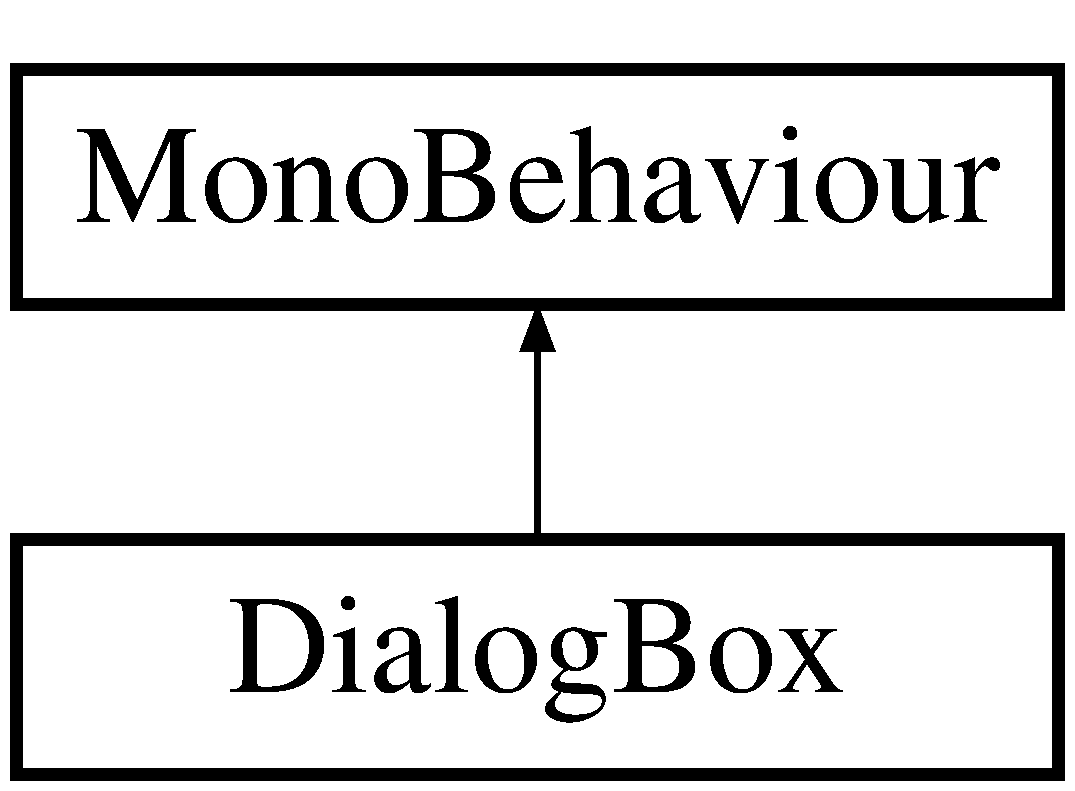
\includegraphics[height=2.000000cm]{class_dialog_box}
\end{center}
\end{figure}
\subsection*{Public Member Functions}
\begin{DoxyCompactItemize}
\item 
void {\bf Show} (string text)
\begin{DoxyCompactList}\small\item\em Show the specified text. \end{DoxyCompactList}\item 
void {\bf On\+Okay} ()
\begin{DoxyCompactList}\small\item\em Action to perform when okay is clicked. \end{DoxyCompactList}\end{DoxyCompactItemize}
\subsection*{Public Attributes}
\begin{DoxyCompactItemize}
\item 
Text {\bf my\+Text}
\begin{DoxyCompactList}\small\item\em My text to display to the user. \end{DoxyCompactList}\end{DoxyCompactItemize}


\subsection{Detailed Description}
A Dialog Box used to display text to the user. 



\subsection{Member Function Documentation}
\index{Dialog\+Box@{Dialog\+Box}!On\+Okay@{On\+Okay}}
\index{On\+Okay@{On\+Okay}!Dialog\+Box@{Dialog\+Box}}
\subsubsection[{On\+Okay()}]{\setlength{\rightskip}{0pt plus 5cm}void Dialog\+Box.\+On\+Okay (
\begin{DoxyParamCaption}
{}
\end{DoxyParamCaption}
)}\label{class_dialog_box_aa639f926939b142fda80df1df7dd8099}


Action to perform when okay is clicked. 

\index{Dialog\+Box@{Dialog\+Box}!Show@{Show}}
\index{Show@{Show}!Dialog\+Box@{Dialog\+Box}}
\subsubsection[{Show(string text)}]{\setlength{\rightskip}{0pt plus 5cm}void Dialog\+Box.\+Show (
\begin{DoxyParamCaption}
\item[{string}]{text}
\end{DoxyParamCaption}
)}\label{class_dialog_box_ae7bb70f489704a901fb2de4115501c59}


Show the specified text. 


\begin{DoxyParams}{Parameters}
{\em text} & The text to display.\\
\hline
\end{DoxyParams}


\subsection{Member Data Documentation}
\index{Dialog\+Box@{Dialog\+Box}!my\+Text@{my\+Text}}
\index{my\+Text@{my\+Text}!Dialog\+Box@{Dialog\+Box}}
\subsubsection[{my\+Text}]{\setlength{\rightskip}{0pt plus 5cm}Text Dialog\+Box.\+my\+Text}\label{class_dialog_box_ab844ea3cf0c1fb85617853ce9d8161ef}


My text to display to the user. 



The documentation for this class was generated from the following file\+:\begin{DoxyCompactItemize}
\item 
Dialog\+Box.\+cs\end{DoxyCompactItemize}

\section{Hand\+On\+Page Class Reference}
\label{class_hand_on_page}\index{Hand\+On\+Page@{Hand\+On\+Page}}


Controls page movement animation  


Inheritance diagram for Hand\+On\+Page\+:\begin{figure}[H]
\begin{center}
\leavevmode
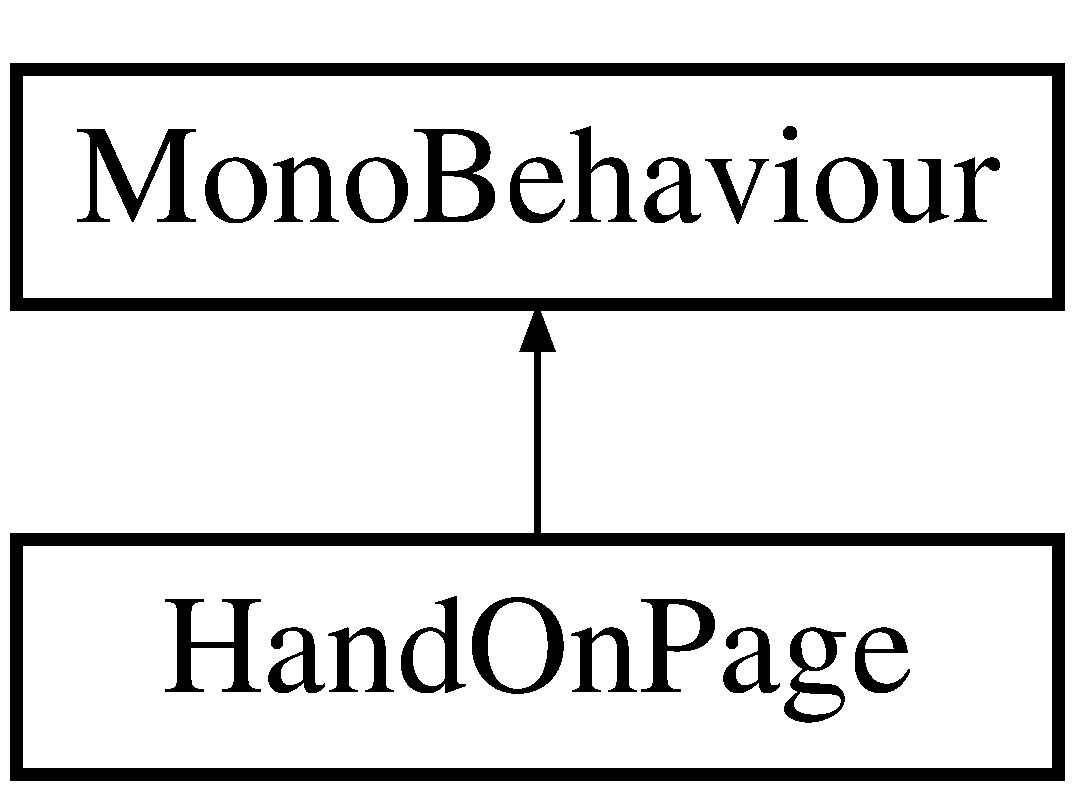
\includegraphics[height=2.000000cm]{class_hand_on_page}
\end{center}
\end{figure}
\subsection*{Public Attributes}
\begin{DoxyCompactItemize}
\item 
Animator {\bf animator}
\begin{DoxyCompactList}\small\item\em The animator of the page. \end{DoxyCompactList}\item 
Collider {\bf page}
\begin{DoxyCompactList}\small\item\em The Collider of the page. \end{DoxyCompactList}\item 
{\bf Page\+Images} {\bf page\+Images}
\begin{DoxyCompactList}\small\item\em The presenter of the I\+I\+IF images. \end{DoxyCompactList}\item 
float {\bf page\+Width}
\begin{DoxyCompactList}\small\item\em The width of the page. \end{DoxyCompactList}\item 
bool {\bf is\+Right}
\begin{DoxyCompactList}\small\item\em Is this the right page? \end{DoxyCompactList}\item 
Renderer[$\,$] {\bf others}
\begin{DoxyCompactList}\small\item\em Pages to hide when this page is over them \end{DoxyCompactList}\end{DoxyCompactItemize}


\subsection{Detailed Description}
Controls page movement animation 



\subsection{Member Data Documentation}
\index{Hand\+On\+Page@{Hand\+On\+Page}!animator@{animator}}
\index{animator@{animator}!Hand\+On\+Page@{Hand\+On\+Page}}
\subsubsection[{animator}]{\setlength{\rightskip}{0pt plus 5cm}Animator Hand\+On\+Page.\+animator}\label{class_hand_on_page_afd57c043c682cf1a01b36c958db9ed18}


The animator of the page. 

\index{Hand\+On\+Page@{Hand\+On\+Page}!is\+Right@{is\+Right}}
\index{is\+Right@{is\+Right}!Hand\+On\+Page@{Hand\+On\+Page}}
\subsubsection[{is\+Right}]{\setlength{\rightskip}{0pt plus 5cm}bool Hand\+On\+Page.\+is\+Right}\label{class_hand_on_page_aeceb11ff110761c6b8de17f6e3db949a}


Is this the right page? 

\index{Hand\+On\+Page@{Hand\+On\+Page}!others@{others}}
\index{others@{others}!Hand\+On\+Page@{Hand\+On\+Page}}
\subsubsection[{others}]{\setlength{\rightskip}{0pt plus 5cm}Renderer [$\,$] Hand\+On\+Page.\+others}\label{class_hand_on_page_a8bf4890b1cca8d94dba8b1e1ab3954e6}


Pages to hide when this page is over them 

\index{Hand\+On\+Page@{Hand\+On\+Page}!page@{page}}
\index{page@{page}!Hand\+On\+Page@{Hand\+On\+Page}}
\subsubsection[{page}]{\setlength{\rightskip}{0pt plus 5cm}Collider Hand\+On\+Page.\+page}\label{class_hand_on_page_a03b366b79c9b970430e0318dd04f98e0}


The Collider of the page. 

\index{Hand\+On\+Page@{Hand\+On\+Page}!page\+Images@{page\+Images}}
\index{page\+Images@{page\+Images}!Hand\+On\+Page@{Hand\+On\+Page}}
\subsubsection[{page\+Images}]{\setlength{\rightskip}{0pt plus 5cm}{\bf Page\+Images} Hand\+On\+Page.\+page\+Images}\label{class_hand_on_page_a700380202f1cfd8554dfa85f918e16e8}


The presenter of the I\+I\+IF images. 

\index{Hand\+On\+Page@{Hand\+On\+Page}!page\+Width@{page\+Width}}
\index{page\+Width@{page\+Width}!Hand\+On\+Page@{Hand\+On\+Page}}
\subsubsection[{page\+Width}]{\setlength{\rightskip}{0pt plus 5cm}float Hand\+On\+Page.\+page\+Width}\label{class_hand_on_page_a83cc71512d2e86c90822af22ce14943d}


The width of the page. 



The documentation for this class was generated from the following file\+:\begin{DoxyCompactItemize}
\item 
Hand\+On\+Page.\+cs\end{DoxyCompactItemize}

\section{Assembly\+C\+Sharp.\+I\+I\+I\+F\+Get\+Manifest Class Reference}
\label{class_assembly_c_sharp_1_1_i_i_i_f_get_manifest}\index{Assembly\+C\+Sharp.\+I\+I\+I\+F\+Get\+Manifest@{Assembly\+C\+Sharp.\+I\+I\+I\+F\+Get\+Manifest}}


Gets the manifest for a I\+I\+IF manuscript.  


\subsection*{Public Member Functions}
\begin{DoxyCompactItemize}
\item 
void {\bf download} (string url)
\begin{DoxyCompactList}\small\item\em Download the manifest from a specified url. \end{DoxyCompactList}\item 
string {\bf get\+Page} (int index)
\begin{DoxyCompactList}\small\item\em Get the url of a specified page. \end{DoxyCompactList}\item 
int {\bf get\+Num\+Of\+Pages} ()
\begin{DoxyCompactList}\small\item\em Gets the number of pages. \end{DoxyCompactList}\end{DoxyCompactItemize}


\subsection{Detailed Description}
Gets the manifest for a I\+I\+IF manuscript. 



\subsection{Member Function Documentation}
\index{Assembly\+C\+Sharp\+::\+I\+I\+I\+F\+Get\+Manifest@{Assembly\+C\+Sharp\+::\+I\+I\+I\+F\+Get\+Manifest}!download@{download}}
\index{download@{download}!Assembly\+C\+Sharp\+::\+I\+I\+I\+F\+Get\+Manifest@{Assembly\+C\+Sharp\+::\+I\+I\+I\+F\+Get\+Manifest}}
\subsubsection[{download(string url)}]{\setlength{\rightskip}{0pt plus 5cm}void Assembly\+C\+Sharp.\+I\+I\+I\+F\+Get\+Manifest.\+download (
\begin{DoxyParamCaption}
\item[{string}]{url}
\end{DoxyParamCaption}
)}\label{class_assembly_c_sharp_1_1_i_i_i_f_get_manifest_adec3122dc016bb1a71088a1f3ed5a760}


Download the manifest from a specified url. 


\begin{DoxyParams}{Parameters}
{\em url} & The U\+RL to download the I\+I\+IF manifest from.\\
\hline
\end{DoxyParams}
\index{Assembly\+C\+Sharp\+::\+I\+I\+I\+F\+Get\+Manifest@{Assembly\+C\+Sharp\+::\+I\+I\+I\+F\+Get\+Manifest}!get\+Num\+Of\+Pages@{get\+Num\+Of\+Pages}}
\index{get\+Num\+Of\+Pages@{get\+Num\+Of\+Pages}!Assembly\+C\+Sharp\+::\+I\+I\+I\+F\+Get\+Manifest@{Assembly\+C\+Sharp\+::\+I\+I\+I\+F\+Get\+Manifest}}
\subsubsection[{get\+Num\+Of\+Pages()}]{\setlength{\rightskip}{0pt plus 5cm}int Assembly\+C\+Sharp.\+I\+I\+I\+F\+Get\+Manifest.\+get\+Num\+Of\+Pages (
\begin{DoxyParamCaption}
{}
\end{DoxyParamCaption}
)}\label{class_assembly_c_sharp_1_1_i_i_i_f_get_manifest_a36f4b3870d7e913b9181b97b2e384707}


Gets the number of pages. 

\begin{DoxyReturn}{Returns}
The number of pages.
\end{DoxyReturn}
\index{Assembly\+C\+Sharp\+::\+I\+I\+I\+F\+Get\+Manifest@{Assembly\+C\+Sharp\+::\+I\+I\+I\+F\+Get\+Manifest}!get\+Page@{get\+Page}}
\index{get\+Page@{get\+Page}!Assembly\+C\+Sharp\+::\+I\+I\+I\+F\+Get\+Manifest@{Assembly\+C\+Sharp\+::\+I\+I\+I\+F\+Get\+Manifest}}
\subsubsection[{get\+Page(int index)}]{\setlength{\rightskip}{0pt plus 5cm}string Assembly\+C\+Sharp.\+I\+I\+I\+F\+Get\+Manifest.\+get\+Page (
\begin{DoxyParamCaption}
\item[{int}]{index}
\end{DoxyParamCaption}
)}\label{class_assembly_c_sharp_1_1_i_i_i_f_get_manifest_a363267d41e370600e961c276a620eb31}


Get the url of a specified page. 

\begin{DoxyReturn}{Returns}
The page url.
\end{DoxyReturn}

\begin{DoxyParams}{Parameters}
{\em index} & The index of the page.\\
\hline
\end{DoxyParams}


The documentation for this class was generated from the following file\+:\begin{DoxyCompactItemize}
\item 
I\+I\+I\+F\+Get\+Manifest.\+cs\end{DoxyCompactItemize}

\section{I\+I\+I\+F\+Image\+Get Class Reference}
\label{class_i_i_i_f_image_get}\index{I\+I\+I\+F\+Image\+Get@{I\+I\+I\+F\+Image\+Get}}


Retrieves an image from an I\+I\+IF server.  


Inheritance diagram for I\+I\+I\+F\+Image\+Get\+:\begin{figure}[H]
\begin{center}
\leavevmode
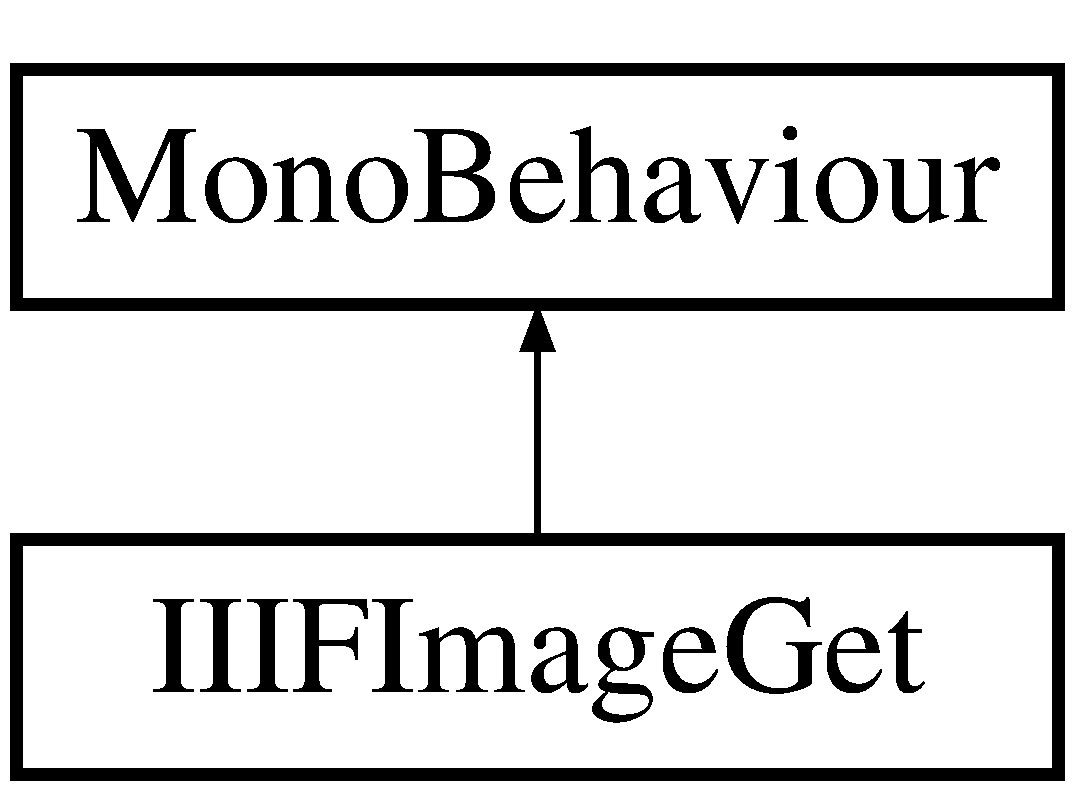
\includegraphics[height=2.000000cm]{class_i_i_i_f_image_get}
\end{center}
\end{figure}
\subsection*{Public Member Functions}
\begin{DoxyCompactItemize}
\item 
I\+Enumerator {\bf Update\+Image} ()
\begin{DoxyCompactList}\small\item\em Updates the image. \end{DoxyCompactList}\item 
string {\bf remove\+Tail} (string new\+Address)
\begin{DoxyCompactList}\small\item\em Removes the tail from a web address. \end{DoxyCompactList}\item 
void {\bf change\+Address} (string new\+Address)
\begin{DoxyCompactList}\small\item\em Changes the web address. \end{DoxyCompactList}\item 
string {\bf get\+Address} ()
\begin{DoxyCompactList}\small\item\em Calculates the web address for the I\+I\+IF image with this \doxyref{I\+I\+I\+F\+Image\+Get}{p.}{class_i_i_i_f_image_get}\textquotesingle{}s settings. \end{DoxyCompactList}\item 
float {\bf Get\+Progress} ()
\begin{DoxyCompactList}\small\item\em Gets the current percentage downloaded of the image. \end{DoxyCompactList}\end{DoxyCompactItemize}
\subsection*{Public Attributes}
\begin{DoxyCompactItemize}
\item 
string {\bf web\+Address}
\begin{DoxyCompactList}\small\item\em The root web address to get the image from. \end{DoxyCompactList}\item 
int {\bf crop\+OffsetX} = -\/1
\begin{DoxyCompactList}\small\item\em The horizontal crop offset. -\/1 If not used. \end{DoxyCompactList}\item 
int {\bf crop\+OffsetY} = -\/1
\begin{DoxyCompactList}\small\item\em The vertical crop offset. \end{DoxyCompactList}\item 
int {\bf crop\+Width} = -\/1
\begin{DoxyCompactList}\small\item\em The width of the crop. \end{DoxyCompactList}\item 
int {\bf crop\+Height} = -\/1
\begin{DoxyCompactList}\small\item\em The height of the crop. \end{DoxyCompactList}\item 
int {\bf target\+Width}
\begin{DoxyCompactList}\small\item\em The width of the target image. \end{DoxyCompactList}\item 
int {\bf target\+Height} = -\/1
\begin{DoxyCompactList}\small\item\em The height of the target image. \end{DoxyCompactList}\item 
bool {\bf mirrored} = false
\begin{DoxyCompactList}\small\item\em Is the image reflected?. \end{DoxyCompactList}\item 
int {\bf rotation} = 0
\begin{DoxyCompactList}\small\item\em The rotation of the image. \end{DoxyCompactList}\item 
string {\bf quality} = \char`\"{}default\char`\"{}
\begin{DoxyCompactList}\small\item\em The quality of the image. \end{DoxyCompactList}\item 
string {\bf format} = \char`\"{}.jpg\char`\"{}
\begin{DoxyCompactList}\small\item\em The format of the image. \end{DoxyCompactList}\item 
Texture2D {\bf texture}
\begin{DoxyCompactList}\small\item\em The image obtained from the I\+I\+IF server. \end{DoxyCompactList}\end{DoxyCompactItemize}


\subsection{Detailed Description}
Retrieves an image from an I\+I\+IF server. 



\subsection{Member Function Documentation}
\index{I\+I\+I\+F\+Image\+Get@{I\+I\+I\+F\+Image\+Get}!change\+Address@{change\+Address}}
\index{change\+Address@{change\+Address}!I\+I\+I\+F\+Image\+Get@{I\+I\+I\+F\+Image\+Get}}
\subsubsection[{change\+Address(string new\+Address)}]{\setlength{\rightskip}{0pt plus 5cm}void I\+I\+I\+F\+Image\+Get.\+change\+Address (
\begin{DoxyParamCaption}
\item[{string}]{new\+Address}
\end{DoxyParamCaption}
)}\label{class_i_i_i_f_image_get_ae312ad6a713e6d7cee3210db59838f00}


Changes the web address. 


\begin{DoxyParams}{Parameters}
{\em new\+Address} & The new web address (still with the tail).\\
\hline
\end{DoxyParams}
\index{I\+I\+I\+F\+Image\+Get@{I\+I\+I\+F\+Image\+Get}!get\+Address@{get\+Address}}
\index{get\+Address@{get\+Address}!I\+I\+I\+F\+Image\+Get@{I\+I\+I\+F\+Image\+Get}}
\subsubsection[{get\+Address()}]{\setlength{\rightskip}{0pt plus 5cm}string I\+I\+I\+F\+Image\+Get.\+get\+Address (
\begin{DoxyParamCaption}
{}
\end{DoxyParamCaption}
)}\label{class_i_i_i_f_image_get_af37d0e78a9db92c63e1f04e3589f05b1}


Calculates the web address for the I\+I\+IF image with this \doxyref{I\+I\+I\+F\+Image\+Get}{p.}{class_i_i_i_f_image_get}\textquotesingle{}s settings. 

\begin{DoxyReturn}{Returns}
The I\+I\+IF web address corresponding to this \doxyref{I\+I\+I\+F\+Image\+Get}{p.}{class_i_i_i_f_image_get}.
\end{DoxyReturn}
\index{I\+I\+I\+F\+Image\+Get@{I\+I\+I\+F\+Image\+Get}!Get\+Progress@{Get\+Progress}}
\index{Get\+Progress@{Get\+Progress}!I\+I\+I\+F\+Image\+Get@{I\+I\+I\+F\+Image\+Get}}
\subsubsection[{Get\+Progress()}]{\setlength{\rightskip}{0pt plus 5cm}float I\+I\+I\+F\+Image\+Get.\+Get\+Progress (
\begin{DoxyParamCaption}
{}
\end{DoxyParamCaption}
)}\label{class_i_i_i_f_image_get_af36dc447c2e08becce3eb0946b7372ec}


Gets the current percentage downloaded of the image. 

\begin{DoxyReturn}{Returns}
The percentage downloaded of the image thus far. 1.\+0f if the image is downloaded.
\end{DoxyReturn}
\index{I\+I\+I\+F\+Image\+Get@{I\+I\+I\+F\+Image\+Get}!remove\+Tail@{remove\+Tail}}
\index{remove\+Tail@{remove\+Tail}!I\+I\+I\+F\+Image\+Get@{I\+I\+I\+F\+Image\+Get}}
\subsubsection[{remove\+Tail(string new\+Address)}]{\setlength{\rightskip}{0pt plus 5cm}string I\+I\+I\+F\+Image\+Get.\+remove\+Tail (
\begin{DoxyParamCaption}
\item[{string}]{new\+Address}
\end{DoxyParamCaption}
)}\label{class_i_i_i_f_image_get_aabc551661bd940d1a06c99074d3cd759}


Removes the tail from a web address. 

\begin{DoxyReturn}{Returns}
The web address with the tail removed.
\end{DoxyReturn}

\begin{DoxyParams}{Parameters}
{\em new\+Address} & The web address to remove the tail from.\\
\hline
\end{DoxyParams}
\index{I\+I\+I\+F\+Image\+Get@{I\+I\+I\+F\+Image\+Get}!Update\+Image@{Update\+Image}}
\index{Update\+Image@{Update\+Image}!I\+I\+I\+F\+Image\+Get@{I\+I\+I\+F\+Image\+Get}}
\subsubsection[{Update\+Image()}]{\setlength{\rightskip}{0pt plus 5cm}I\+Enumerator I\+I\+I\+F\+Image\+Get.\+Update\+Image (
\begin{DoxyParamCaption}
{}
\end{DoxyParamCaption}
)}\label{class_i_i_i_f_image_get_a2f44ae11571a424cb7e6b473036577a3}


Updates the image. 



\subsection{Member Data Documentation}
\index{I\+I\+I\+F\+Image\+Get@{I\+I\+I\+F\+Image\+Get}!crop\+Height@{crop\+Height}}
\index{crop\+Height@{crop\+Height}!I\+I\+I\+F\+Image\+Get@{I\+I\+I\+F\+Image\+Get}}
\subsubsection[{crop\+Height}]{\setlength{\rightskip}{0pt plus 5cm}int I\+I\+I\+F\+Image\+Get.\+crop\+Height = -\/1}\label{class_i_i_i_f_image_get_a9db467afe54453d71953d79d09ccd856}


The height of the crop. 

\index{I\+I\+I\+F\+Image\+Get@{I\+I\+I\+F\+Image\+Get}!crop\+OffsetX@{crop\+OffsetX}}
\index{crop\+OffsetX@{crop\+OffsetX}!I\+I\+I\+F\+Image\+Get@{I\+I\+I\+F\+Image\+Get}}
\subsubsection[{crop\+OffsetX}]{\setlength{\rightskip}{0pt plus 5cm}int I\+I\+I\+F\+Image\+Get.\+crop\+OffsetX = -\/1}\label{class_i_i_i_f_image_get_a3e424fce3d74529b87b488a4a918da64}


The horizontal crop offset. -\/1 If not used. 

\index{I\+I\+I\+F\+Image\+Get@{I\+I\+I\+F\+Image\+Get}!crop\+OffsetY@{crop\+OffsetY}}
\index{crop\+OffsetY@{crop\+OffsetY}!I\+I\+I\+F\+Image\+Get@{I\+I\+I\+F\+Image\+Get}}
\subsubsection[{crop\+OffsetY}]{\setlength{\rightskip}{0pt plus 5cm}int I\+I\+I\+F\+Image\+Get.\+crop\+OffsetY = -\/1}\label{class_i_i_i_f_image_get_ab21f44619cba32ab34a99723f4e2c21e}


The vertical crop offset. 

\index{I\+I\+I\+F\+Image\+Get@{I\+I\+I\+F\+Image\+Get}!crop\+Width@{crop\+Width}}
\index{crop\+Width@{crop\+Width}!I\+I\+I\+F\+Image\+Get@{I\+I\+I\+F\+Image\+Get}}
\subsubsection[{crop\+Width}]{\setlength{\rightskip}{0pt plus 5cm}int I\+I\+I\+F\+Image\+Get.\+crop\+Width = -\/1}\label{class_i_i_i_f_image_get_ab88ed28d3c28596fbd0f61ed53551bba}


The width of the crop. 

\index{I\+I\+I\+F\+Image\+Get@{I\+I\+I\+F\+Image\+Get}!format@{format}}
\index{format@{format}!I\+I\+I\+F\+Image\+Get@{I\+I\+I\+F\+Image\+Get}}
\subsubsection[{format}]{\setlength{\rightskip}{0pt plus 5cm}string I\+I\+I\+F\+Image\+Get.\+format = \char`\"{}.jpg\char`\"{}}\label{class_i_i_i_f_image_get_a816a7c3831777caa0bf2c314dc9e3d2b}


The format of the image. 

\index{I\+I\+I\+F\+Image\+Get@{I\+I\+I\+F\+Image\+Get}!mirrored@{mirrored}}
\index{mirrored@{mirrored}!I\+I\+I\+F\+Image\+Get@{I\+I\+I\+F\+Image\+Get}}
\subsubsection[{mirrored}]{\setlength{\rightskip}{0pt plus 5cm}bool I\+I\+I\+F\+Image\+Get.\+mirrored = false}\label{class_i_i_i_f_image_get_a8ca420b349df804f1dd087cfdaa389e4}


Is the image reflected?. 

\index{I\+I\+I\+F\+Image\+Get@{I\+I\+I\+F\+Image\+Get}!quality@{quality}}
\index{quality@{quality}!I\+I\+I\+F\+Image\+Get@{I\+I\+I\+F\+Image\+Get}}
\subsubsection[{quality}]{\setlength{\rightskip}{0pt plus 5cm}string I\+I\+I\+F\+Image\+Get.\+quality = \char`\"{}default\char`\"{}}\label{class_i_i_i_f_image_get_a0edb84f6ed8c3618bfbcb5383403f756}


The quality of the image. 

\index{I\+I\+I\+F\+Image\+Get@{I\+I\+I\+F\+Image\+Get}!rotation@{rotation}}
\index{rotation@{rotation}!I\+I\+I\+F\+Image\+Get@{I\+I\+I\+F\+Image\+Get}}
\subsubsection[{rotation}]{\setlength{\rightskip}{0pt plus 5cm}int I\+I\+I\+F\+Image\+Get.\+rotation = 0}\label{class_i_i_i_f_image_get_a4cdbf0a334d0be4334c00a2cb6eb26c1}


The rotation of the image. 

\index{I\+I\+I\+F\+Image\+Get@{I\+I\+I\+F\+Image\+Get}!target\+Height@{target\+Height}}
\index{target\+Height@{target\+Height}!I\+I\+I\+F\+Image\+Get@{I\+I\+I\+F\+Image\+Get}}
\subsubsection[{target\+Height}]{\setlength{\rightskip}{0pt plus 5cm}int I\+I\+I\+F\+Image\+Get.\+target\+Height = -\/1}\label{class_i_i_i_f_image_get_a81ec0146df6843169c7a301d0018b29b}


The height of the target image. 

\index{I\+I\+I\+F\+Image\+Get@{I\+I\+I\+F\+Image\+Get}!target\+Width@{target\+Width}}
\index{target\+Width@{target\+Width}!I\+I\+I\+F\+Image\+Get@{I\+I\+I\+F\+Image\+Get}}
\subsubsection[{target\+Width}]{\setlength{\rightskip}{0pt plus 5cm}int I\+I\+I\+F\+Image\+Get.\+target\+Width}\label{class_i_i_i_f_image_get_ad29efbe7f08cd76fa519aa5ca036c404}


The width of the target image. 

\index{I\+I\+I\+F\+Image\+Get@{I\+I\+I\+F\+Image\+Get}!texture@{texture}}
\index{texture@{texture}!I\+I\+I\+F\+Image\+Get@{I\+I\+I\+F\+Image\+Get}}
\subsubsection[{texture}]{\setlength{\rightskip}{0pt plus 5cm}Texture2D I\+I\+I\+F\+Image\+Get.\+texture}\label{class_i_i_i_f_image_get_acd964c8562547558f31bfc04ff434565}


The image obtained from the I\+I\+IF server. 

\index{I\+I\+I\+F\+Image\+Get@{I\+I\+I\+F\+Image\+Get}!web\+Address@{web\+Address}}
\index{web\+Address@{web\+Address}!I\+I\+I\+F\+Image\+Get@{I\+I\+I\+F\+Image\+Get}}
\subsubsection[{web\+Address}]{\setlength{\rightskip}{0pt plus 5cm}string I\+I\+I\+F\+Image\+Get.\+web\+Address}\label{class_i_i_i_f_image_get_a4b3539da1bc9765bae28166cbe13bdfb}


The root web address to get the image from. 



The documentation for this class was generated from the following file\+:\begin{DoxyCompactItemize}
\item 
I\+I\+I\+F\+Image\+Get.\+cs\end{DoxyCompactItemize}

\section{I\+I\+I\+F\+Image\+Loading\+Bar Class Reference}
\label{class_i_i_i_f_image_loading_bar}\index{I\+I\+I\+F\+Image\+Loading\+Bar@{I\+I\+I\+F\+Image\+Loading\+Bar}}


The loading bar for an I\+I\+IF image.  


Inheritance diagram for I\+I\+I\+F\+Image\+Loading\+Bar\+:\begin{figure}[H]
\begin{center}
\leavevmode
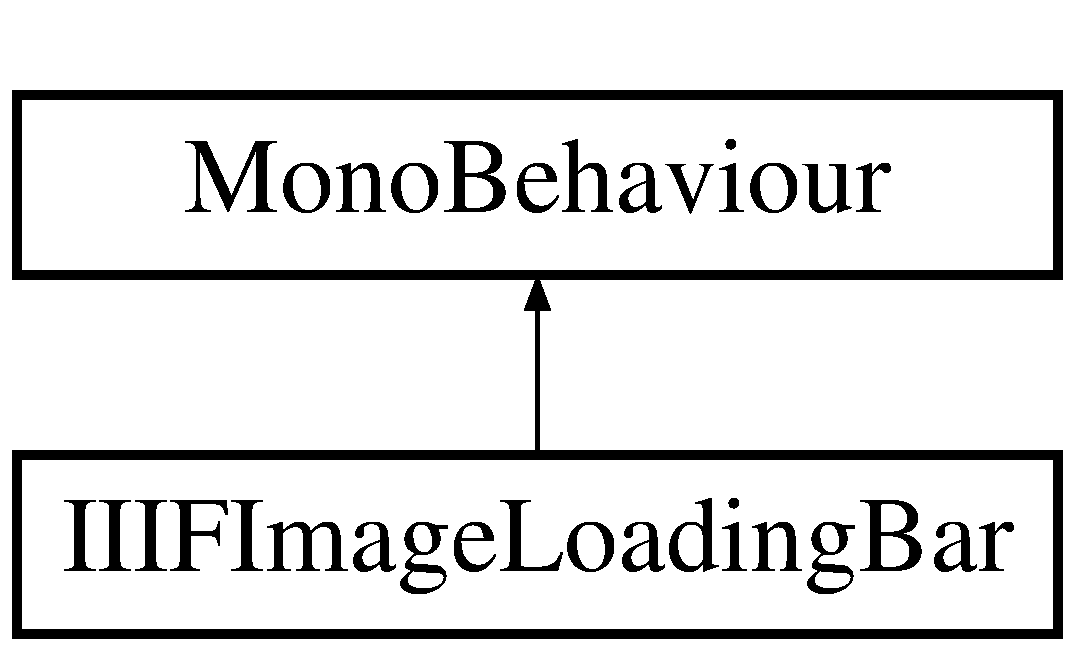
\includegraphics[height=2.000000cm]{class_i_i_i_f_image_loading_bar}
\end{center}
\end{figure}
\subsection*{Public Attributes}
\begin{DoxyCompactItemize}
\item 
{\bf I\+I\+I\+F\+Image\+Get} {\bf image}
\begin{DoxyCompactList}\small\item\em The image to monitor the download progress of. \end{DoxyCompactList}\item 
Image {\bf back}
\begin{DoxyCompactList}\small\item\em The background of the loading bar. \end{DoxyCompactList}\item 
Image {\bf progress\+Bar}
\begin{DoxyCompactList}\small\item\em The foreground of the loading bar. \end{DoxyCompactList}\end{DoxyCompactItemize}


\subsection{Detailed Description}
The loading bar for an I\+I\+IF image. 



\subsection{Member Data Documentation}
\index{I\+I\+I\+F\+Image\+Loading\+Bar@{I\+I\+I\+F\+Image\+Loading\+Bar}!back@{back}}
\index{back@{back}!I\+I\+I\+F\+Image\+Loading\+Bar@{I\+I\+I\+F\+Image\+Loading\+Bar}}
\subsubsection[{back}]{\setlength{\rightskip}{0pt plus 5cm}Image I\+I\+I\+F\+Image\+Loading\+Bar.\+back}\label{class_i_i_i_f_image_loading_bar_a6dd3836a2b2b5d21ff6350e6a5b75746}


The background of the loading bar. 

\index{I\+I\+I\+F\+Image\+Loading\+Bar@{I\+I\+I\+F\+Image\+Loading\+Bar}!image@{image}}
\index{image@{image}!I\+I\+I\+F\+Image\+Loading\+Bar@{I\+I\+I\+F\+Image\+Loading\+Bar}}
\subsubsection[{image}]{\setlength{\rightskip}{0pt plus 5cm}{\bf I\+I\+I\+F\+Image\+Get} I\+I\+I\+F\+Image\+Loading\+Bar.\+image}\label{class_i_i_i_f_image_loading_bar_a06002000920eb3815de43443a5cf36d1}


The image to monitor the download progress of. 

\index{I\+I\+I\+F\+Image\+Loading\+Bar@{I\+I\+I\+F\+Image\+Loading\+Bar}!progress\+Bar@{progress\+Bar}}
\index{progress\+Bar@{progress\+Bar}!I\+I\+I\+F\+Image\+Loading\+Bar@{I\+I\+I\+F\+Image\+Loading\+Bar}}
\subsubsection[{progress\+Bar}]{\setlength{\rightskip}{0pt plus 5cm}Image I\+I\+I\+F\+Image\+Loading\+Bar.\+progress\+Bar}\label{class_i_i_i_f_image_loading_bar_a4890e8e5a52ec51f2a740d1b77fdf1a9}


The foreground of the loading bar. 



The documentation for this class was generated from the following file\+:\begin{DoxyCompactItemize}
\item 
I\+I\+I\+F\+Image\+Loading\+Bar.\+cs\end{DoxyCompactItemize}

\section{Move Class Reference}
\label{class_move}\index{Move@{Move}}


The movement logic for the book mode camera.  


Inheritance diagram for Move\+:\begin{figure}[H]
\begin{center}
\leavevmode
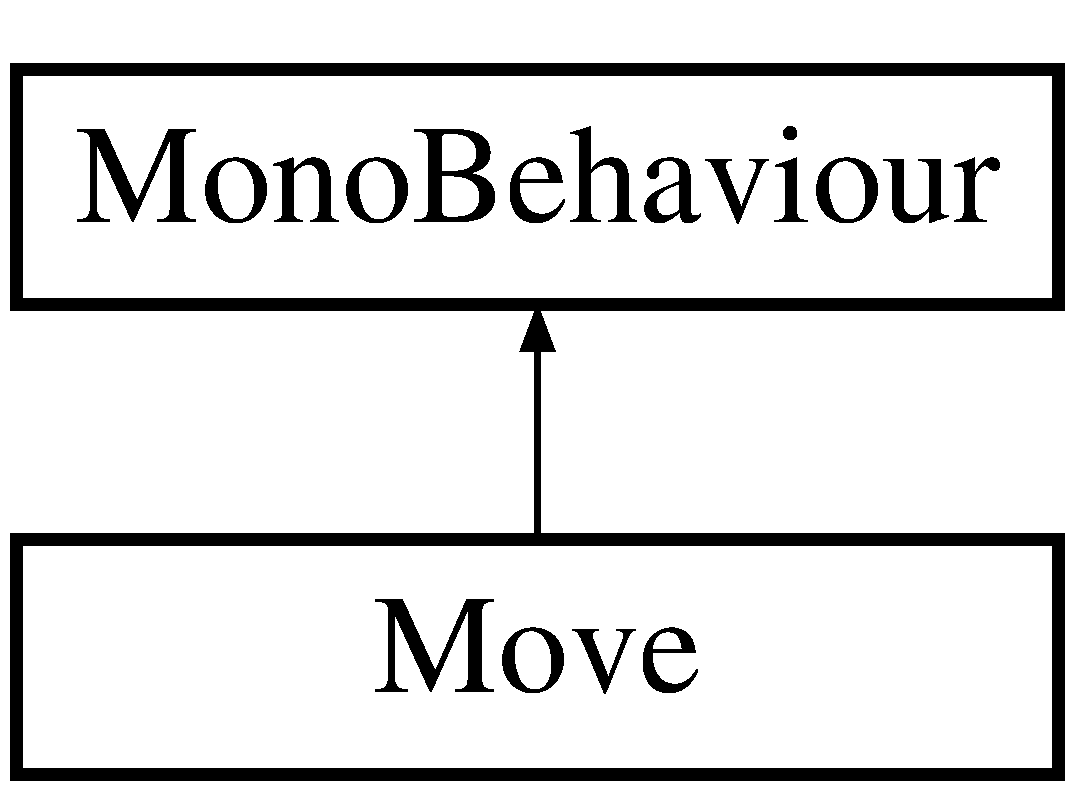
\includegraphics[height=2.000000cm]{class_move}
\end{center}
\end{figure}
\subsection*{Public Member Functions}
\begin{DoxyCompactItemize}
\item 
void {\bf set\+Activated} (bool is\+Activated)
\begin{DoxyCompactList}\small\item\em Enable/\+Disable movement. \end{DoxyCompactList}\end{DoxyCompactItemize}
\subsection*{Public Attributes}
\begin{DoxyCompactItemize}
\item 
Transform {\bf my\+Transform}
\begin{DoxyCompactList}\small\item\em The position of the book mode camera \end{DoxyCompactList}\item 
float {\bf speed}
\begin{DoxyCompactList}\small\item\em The speed of the book mode camera. \end{DoxyCompactList}\end{DoxyCompactItemize}


\subsection{Detailed Description}
The movement logic for the book mode camera. 



\subsection{Member Function Documentation}
\index{Move@{Move}!set\+Activated@{set\+Activated}}
\index{set\+Activated@{set\+Activated}!Move@{Move}}
\subsubsection[{set\+Activated(bool is\+Activated)}]{\setlength{\rightskip}{0pt plus 5cm}void Move.\+set\+Activated (
\begin{DoxyParamCaption}
\item[{bool}]{is\+Activated}
\end{DoxyParamCaption}
)}\label{class_move_af0326636647d755368aa657a5cf97cbe}


Enable/\+Disable movement. 


\begin{DoxyParams}{Parameters}
{\em is\+Activated} & If set to {\ttfamily true} enables movement. Else, disables movement.\\
\hline
\end{DoxyParams}


\subsection{Member Data Documentation}
\index{Move@{Move}!my\+Transform@{my\+Transform}}
\index{my\+Transform@{my\+Transform}!Move@{Move}}
\subsubsection[{my\+Transform}]{\setlength{\rightskip}{0pt plus 5cm}Transform Move.\+my\+Transform}\label{class_move_a37d9e5e6fba0c218526752d9cca34a3a}


The position of the book mode camera 

\index{Move@{Move}!speed@{speed}}
\index{speed@{speed}!Move@{Move}}
\subsubsection[{speed}]{\setlength{\rightskip}{0pt plus 5cm}float Move.\+speed}\label{class_move_ad3bff9bc14f0e22d33fe5b5b5d9b58b1}


The speed of the book mode camera. 



The documentation for this class was generated from the following file\+:\begin{DoxyCompactItemize}
\item 
Move.\+cs\end{DoxyCompactItemize}

\section{Move\+Player Class Reference}
\label{class_move_player}\index{Move\+Player@{Move\+Player}}


Movement logic for the navigation mode camera  


Inheritance diagram for Move\+Player\+:\begin{figure}[H]
\begin{center}
\leavevmode
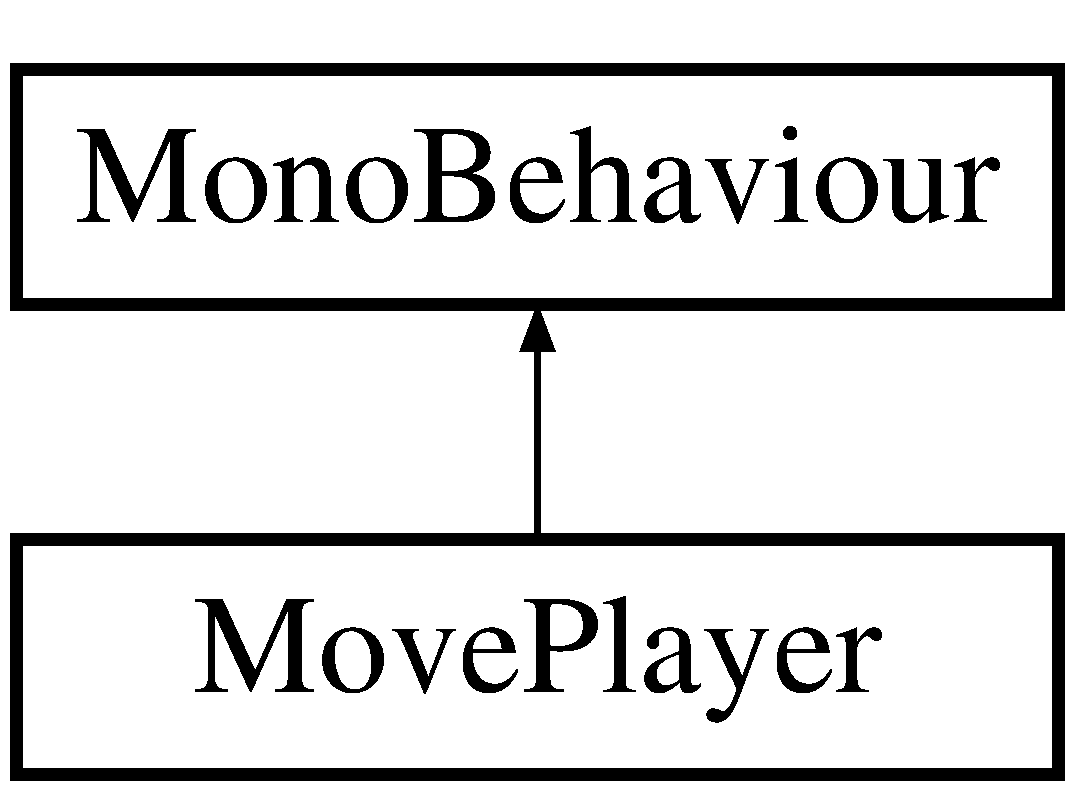
\includegraphics[height=2.000000cm]{class_move_player}
\end{center}
\end{figure}
\subsection*{Public Member Functions}
\begin{DoxyCompactItemize}
\item 
void {\bf Change\+Control} (bool new\+Control)
\begin{DoxyCompactList}\small\item\em Enables/\+Disables movement. \end{DoxyCompactList}\end{DoxyCompactItemize}
\subsection*{Public Attributes}
\begin{DoxyCompactItemize}
\item 
Mono\+Behaviour {\bf move\+Script}
\begin{DoxyCompactList}\small\item\em The script that controls the player. \end{DoxyCompactList}\item 
bool {\bf in\+Control}
\begin{DoxyCompactList}\small\item\em Is the player in navigation mode? \end{DoxyCompactList}\end{DoxyCompactItemize}


\subsection{Detailed Description}
Movement logic for the navigation mode camera 



\subsection{Member Function Documentation}
\index{Move\+Player@{Move\+Player}!Change\+Control@{Change\+Control}}
\index{Change\+Control@{Change\+Control}!Move\+Player@{Move\+Player}}
\subsubsection[{Change\+Control(bool new\+Control)}]{\setlength{\rightskip}{0pt plus 5cm}void Move\+Player.\+Change\+Control (
\begin{DoxyParamCaption}
\item[{bool}]{new\+Control}
\end{DoxyParamCaption}
)}\label{class_move_player_abd1c84d23f1a93c79e26f9cf6e495aa8}


Enables/\+Disables movement. 


\begin{DoxyParams}{Parameters}
{\em new\+Control} & If set to {\ttfamily true} enables movement. Otherwise, disables movements.\\
\hline
\end{DoxyParams}


\subsection{Member Data Documentation}
\index{Move\+Player@{Move\+Player}!in\+Control@{in\+Control}}
\index{in\+Control@{in\+Control}!Move\+Player@{Move\+Player}}
\subsubsection[{in\+Control}]{\setlength{\rightskip}{0pt plus 5cm}bool Move\+Player.\+in\+Control}\label{class_move_player_affaf4ad002a1a2595f8517c92bdb5db7}


Is the player in navigation mode? 

\index{Move\+Player@{Move\+Player}!move\+Script@{move\+Script}}
\index{move\+Script@{move\+Script}!Move\+Player@{Move\+Player}}
\subsubsection[{move\+Script}]{\setlength{\rightskip}{0pt plus 5cm}Mono\+Behaviour Move\+Player.\+move\+Script}\label{class_move_player_ab4f118400fc2b5b9efe4eafe76f62182}


The script that controls the player. 



The documentation for this class was generated from the following file\+:\begin{DoxyCompactItemize}
\item 
Move\+Player.\+cs\end{DoxyCompactItemize}

\section{Move\+Spotlight Class Reference}
\label{class_move_spotlight}\index{Move\+Spotlight@{Move\+Spotlight}}


The controls logic for the spotlight tool.  


Inheritance diagram for Move\+Spotlight\+:\begin{figure}[H]
\begin{center}
\leavevmode
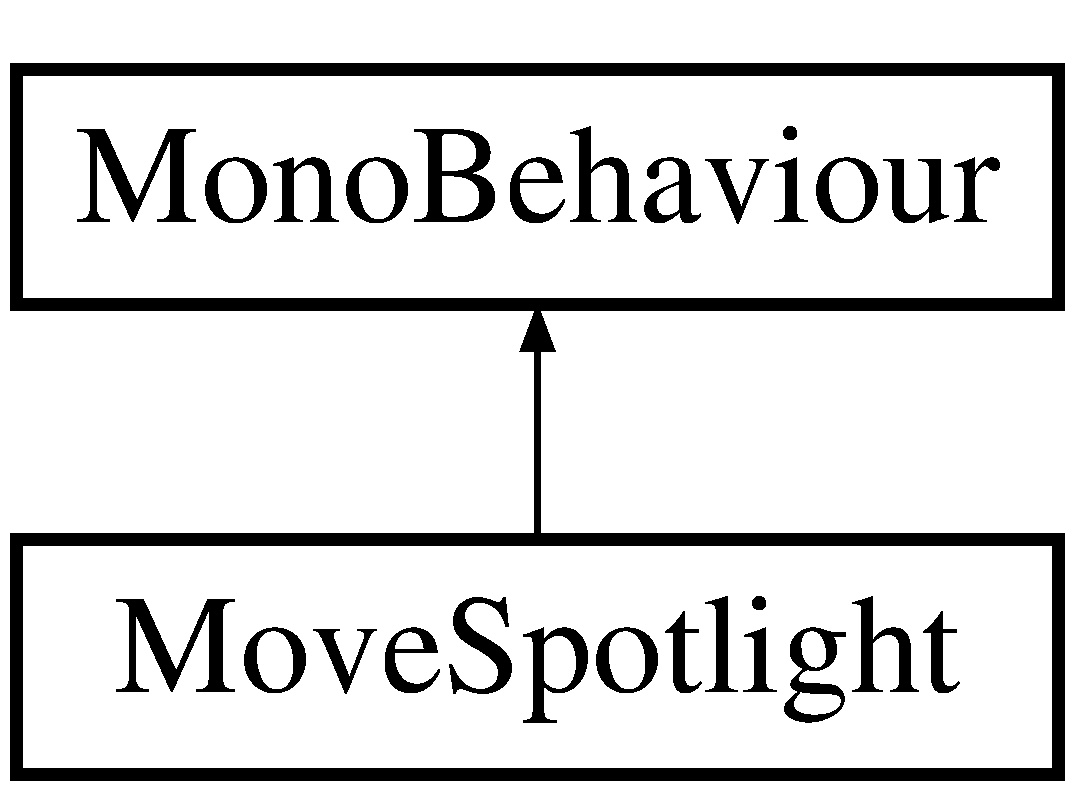
\includegraphics[height=2.000000cm]{class_move_spotlight}
\end{center}
\end{figure}
\subsection*{Public Member Functions}
\begin{DoxyCompactItemize}
\item 
void {\bf update\+Hue} (float hue)
\begin{DoxyCompactList}\small\item\em Updates the hue of the spotlight. \end{DoxyCompactList}\item 
void {\bf update\+Sat} (float sat)
\begin{DoxyCompactList}\small\item\em Updates the saturation of the spotlight. \end{DoxyCompactList}\item 
void {\bf update\+Value} (float value)
\begin{DoxyCompactList}\small\item\em Updates the value of the spotlight. \end{DoxyCompactList}\item 
void {\bf update\+Size} (float new\+Size)
\begin{DoxyCompactList}\small\item\em Updates the size of the spotlight. \end{DoxyCompactList}\item 
void {\bf update\+Brightness} (float brightness)
\begin{DoxyCompactList}\small\item\em Updates the brightness of the spotlight. \end{DoxyCompactList}\item 
void {\bf freeze\+Position} (bool is\+Freeze)
\begin{DoxyCompactList}\small\item\em Freezes/\+Unfreezes the position of the spotlight. \end{DoxyCompactList}\item 
void {\bf hide\+Properties} (bool is\+Hiding)
\begin{DoxyCompactList}\small\item\em Hides/\+Shows the settings of the spotlight. \end{DoxyCompactList}\end{DoxyCompactItemize}
\subsection*{Public Attributes}
\begin{DoxyCompactItemize}
\item 
float {\bf minX}
\begin{DoxyCompactList}\small\item\em The minimum x position. \end{DoxyCompactList}\item 
float {\bf minY}
\begin{DoxyCompactList}\small\item\em The minimum y position. \end{DoxyCompactList}\item 
float {\bf maxX}
\begin{DoxyCompactList}\small\item\em The max x position. \end{DoxyCompactList}\item 
float {\bf maxY}
\begin{DoxyCompactList}\small\item\em The max y position. \end{DoxyCompactList}\item 
Camera {\bf cam}
\begin{DoxyCompactList}\small\item\em The book mode camera \end{DoxyCompactList}\item 
Light {\bf spot\+Light}
\begin{DoxyCompactList}\small\item\em The spot light. \end{DoxyCompactList}\item 
Light {\bf world\+Light}
\begin{DoxyCompactList}\small\item\em The world lighting. \end{DoxyCompactList}\item 
Light {\bf ceiling\+Light}
\begin{DoxyCompactList}\small\item\em The ceiling light. \end{DoxyCompactList}\item 
Image {\bf preview}
\begin{DoxyCompactList}\small\item\em The preview color of the spotlight. \end{DoxyCompactList}\item 
Toggle {\bf frozen\+Toggle}
\begin{DoxyCompactList}\small\item\em The Toggle that controls if this spotlight is frozen. \end{DoxyCompactList}\item 
Toggle {\bf hide\+Toggle}
\begin{DoxyCompactList}\small\item\em The Toggle that controls hiding/showing the settings of this spotlight. \end{DoxyCompactList}\item 
bool {\bf frozen} = false
\begin{DoxyCompactList}\small\item\em Is the spotlight frozen in position? \end{DoxyCompactList}\item 
bool {\bf hiding\+Properties} = false
\begin{DoxyCompactList}\small\item\em Are the settings of this spotlight hidden? \end{DoxyCompactList}\item 
Transform {\bf properties}
\begin{DoxyCompactList}\small\item\em The settings of this spotlight. \end{DoxyCompactList}\end{DoxyCompactItemize}


\subsection{Detailed Description}
The controls logic for the spotlight tool. 



\subsection{Member Function Documentation}
\index{Move\+Spotlight@{Move\+Spotlight}!freeze\+Position@{freeze\+Position}}
\index{freeze\+Position@{freeze\+Position}!Move\+Spotlight@{Move\+Spotlight}}
\subsubsection[{freeze\+Position(bool is\+Freeze)}]{\setlength{\rightskip}{0pt plus 5cm}void Move\+Spotlight.\+freeze\+Position (
\begin{DoxyParamCaption}
\item[{bool}]{is\+Freeze}
\end{DoxyParamCaption}
)}\label{class_move_spotlight_a46b925b55f919f6e86eaa22710d106c1}


Freezes/\+Unfreezes the position of the spotlight. 


\begin{DoxyParams}{Parameters}
{\em is\+Freeze} & If set to {\ttfamily true} freezes the position. Otherwises, unfreezes the position.\\
\hline
\end{DoxyParams}
\index{Move\+Spotlight@{Move\+Spotlight}!hide\+Properties@{hide\+Properties}}
\index{hide\+Properties@{hide\+Properties}!Move\+Spotlight@{Move\+Spotlight}}
\subsubsection[{hide\+Properties(bool is\+Hiding)}]{\setlength{\rightskip}{0pt plus 5cm}void Move\+Spotlight.\+hide\+Properties (
\begin{DoxyParamCaption}
\item[{bool}]{is\+Hiding}
\end{DoxyParamCaption}
)}\label{class_move_spotlight_a62ae8a749a406c3b689063828e6b74e3}


Hides/\+Shows the settings of the spotlight. 


\begin{DoxyParams}{Parameters}
{\em is\+Hiding} & If set to {\ttfamily true} hides the settings. Otherwise, show the settings.\\
\hline
\end{DoxyParams}
\index{Move\+Spotlight@{Move\+Spotlight}!update\+Brightness@{update\+Brightness}}
\index{update\+Brightness@{update\+Brightness}!Move\+Spotlight@{Move\+Spotlight}}
\subsubsection[{update\+Brightness(float brightness)}]{\setlength{\rightskip}{0pt plus 5cm}void Move\+Spotlight.\+update\+Brightness (
\begin{DoxyParamCaption}
\item[{float}]{brightness}
\end{DoxyParamCaption}
)}\label{class_move_spotlight_a52ac982a0b20d11ab96e1c264f40b437}


Updates the brightness of the spotlight. 


\begin{DoxyParams}{Parameters}
{\em brightness} & The new brightness of the spotlight (between 0.\+0f and 1.\+0f).\\
\hline
\end{DoxyParams}
\index{Move\+Spotlight@{Move\+Spotlight}!update\+Hue@{update\+Hue}}
\index{update\+Hue@{update\+Hue}!Move\+Spotlight@{Move\+Spotlight}}
\subsubsection[{update\+Hue(float hue)}]{\setlength{\rightskip}{0pt plus 5cm}void Move\+Spotlight.\+update\+Hue (
\begin{DoxyParamCaption}
\item[{float}]{hue}
\end{DoxyParamCaption}
)}\label{class_move_spotlight_a42e2980f29dbb07819cf8bda8695095b}


Updates the hue of the spotlight. 


\begin{DoxyParams}{Parameters}
{\em hue} & The new hue (between 0.\+0f and 1.\+0f).\\
\hline
\end{DoxyParams}
\index{Move\+Spotlight@{Move\+Spotlight}!update\+Sat@{update\+Sat}}
\index{update\+Sat@{update\+Sat}!Move\+Spotlight@{Move\+Spotlight}}
\subsubsection[{update\+Sat(float sat)}]{\setlength{\rightskip}{0pt plus 5cm}void Move\+Spotlight.\+update\+Sat (
\begin{DoxyParamCaption}
\item[{float}]{sat}
\end{DoxyParamCaption}
)}\label{class_move_spotlight_ac1aa13c1e6ab166fc6eac65216f4f4cb}


Updates the saturation of the spotlight. 


\begin{DoxyParams}{Parameters}
{\em sat} & The new saturation (between 0.\+0f and 1.\+0f).\\
\hline
\end{DoxyParams}
\index{Move\+Spotlight@{Move\+Spotlight}!update\+Size@{update\+Size}}
\index{update\+Size@{update\+Size}!Move\+Spotlight@{Move\+Spotlight}}
\subsubsection[{update\+Size(float new\+Size)}]{\setlength{\rightskip}{0pt plus 5cm}void Move\+Spotlight.\+update\+Size (
\begin{DoxyParamCaption}
\item[{float}]{new\+Size}
\end{DoxyParamCaption}
)}\label{class_move_spotlight_a1a2a859b51a4cc2651127b4ce7f23c69}


Updates the size of the spotlight. 


\begin{DoxyParams}{Parameters}
{\em new\+Size} & New size of the spotlight (between 0.\+0f and 1.\+0f).\\
\hline
\end{DoxyParams}
\index{Move\+Spotlight@{Move\+Spotlight}!update\+Value@{update\+Value}}
\index{update\+Value@{update\+Value}!Move\+Spotlight@{Move\+Spotlight}}
\subsubsection[{update\+Value(float value)}]{\setlength{\rightskip}{0pt plus 5cm}void Move\+Spotlight.\+update\+Value (
\begin{DoxyParamCaption}
\item[{float}]{value}
\end{DoxyParamCaption}
)}\label{class_move_spotlight_acec837332b344a64454afe71bd08eed9}


Updates the value of the spotlight. 


\begin{DoxyParams}{Parameters}
{\em value} & The new value (between 0.\+0f and 1.\+0f).\\
\hline
\end{DoxyParams}


\subsection{Member Data Documentation}
\index{Move\+Spotlight@{Move\+Spotlight}!cam@{cam}}
\index{cam@{cam}!Move\+Spotlight@{Move\+Spotlight}}
\subsubsection[{cam}]{\setlength{\rightskip}{0pt plus 5cm}Camera Move\+Spotlight.\+cam}\label{class_move_spotlight_a0074ba44a6e80eaf5ff4030bc7bd2199}


The book mode camera 

\index{Move\+Spotlight@{Move\+Spotlight}!ceiling\+Light@{ceiling\+Light}}
\index{ceiling\+Light@{ceiling\+Light}!Move\+Spotlight@{Move\+Spotlight}}
\subsubsection[{ceiling\+Light}]{\setlength{\rightskip}{0pt plus 5cm}Light Move\+Spotlight.\+ceiling\+Light}\label{class_move_spotlight_a0db93502d6482412f36571b5a4b99be7}


The ceiling light. 

\index{Move\+Spotlight@{Move\+Spotlight}!frozen@{frozen}}
\index{frozen@{frozen}!Move\+Spotlight@{Move\+Spotlight}}
\subsubsection[{frozen}]{\setlength{\rightskip}{0pt plus 5cm}bool Move\+Spotlight.\+frozen = false}\label{class_move_spotlight_aa22de39a7cf399688b5632b0fa632fa6}


Is the spotlight frozen in position? 

\index{Move\+Spotlight@{Move\+Spotlight}!frozen\+Toggle@{frozen\+Toggle}}
\index{frozen\+Toggle@{frozen\+Toggle}!Move\+Spotlight@{Move\+Spotlight}}
\subsubsection[{frozen\+Toggle}]{\setlength{\rightskip}{0pt plus 5cm}Toggle Move\+Spotlight.\+frozen\+Toggle}\label{class_move_spotlight_ac09eea20cd14e6b07b6097dc7d289acf}


The Toggle that controls if this spotlight is frozen. 

\index{Move\+Spotlight@{Move\+Spotlight}!hide\+Toggle@{hide\+Toggle}}
\index{hide\+Toggle@{hide\+Toggle}!Move\+Spotlight@{Move\+Spotlight}}
\subsubsection[{hide\+Toggle}]{\setlength{\rightskip}{0pt plus 5cm}Toggle Move\+Spotlight.\+hide\+Toggle}\label{class_move_spotlight_a5f4d11791aa7a41bf3742465409469c3}


The Toggle that controls hiding/showing the settings of this spotlight. 

\index{Move\+Spotlight@{Move\+Spotlight}!hiding\+Properties@{hiding\+Properties}}
\index{hiding\+Properties@{hiding\+Properties}!Move\+Spotlight@{Move\+Spotlight}}
\subsubsection[{hiding\+Properties}]{\setlength{\rightskip}{0pt plus 5cm}bool Move\+Spotlight.\+hiding\+Properties = false}\label{class_move_spotlight_a722fb5b9e8a719242a968d730e7341fa}


Are the settings of this spotlight hidden? 

\index{Move\+Spotlight@{Move\+Spotlight}!maxX@{maxX}}
\index{maxX@{maxX}!Move\+Spotlight@{Move\+Spotlight}}
\subsubsection[{maxX}]{\setlength{\rightskip}{0pt plus 5cm}float Move\+Spotlight.\+maxX}\label{class_move_spotlight_affbf3080d9cf95a56d80f1b30b4ee415}


The max x position. 

\index{Move\+Spotlight@{Move\+Spotlight}!maxY@{maxY}}
\index{maxY@{maxY}!Move\+Spotlight@{Move\+Spotlight}}
\subsubsection[{maxY}]{\setlength{\rightskip}{0pt plus 5cm}float Move\+Spotlight.\+maxY}\label{class_move_spotlight_a255c1781f89cb8048d3346d8ed17ee24}


The max y position. 

\index{Move\+Spotlight@{Move\+Spotlight}!minX@{minX}}
\index{minX@{minX}!Move\+Spotlight@{Move\+Spotlight}}
\subsubsection[{minX}]{\setlength{\rightskip}{0pt plus 5cm}float Move\+Spotlight.\+minX}\label{class_move_spotlight_ab6bdcf35eef7c30ed2f43fe359636c06}


The minimum x position. 

\index{Move\+Spotlight@{Move\+Spotlight}!minY@{minY}}
\index{minY@{minY}!Move\+Spotlight@{Move\+Spotlight}}
\subsubsection[{minY}]{\setlength{\rightskip}{0pt plus 5cm}float Move\+Spotlight.\+minY}\label{class_move_spotlight_a791cb5fd988708314ded26cddd7381de}


The minimum y position. 

\index{Move\+Spotlight@{Move\+Spotlight}!preview@{preview}}
\index{preview@{preview}!Move\+Spotlight@{Move\+Spotlight}}
\subsubsection[{preview}]{\setlength{\rightskip}{0pt plus 5cm}Image Move\+Spotlight.\+preview}\label{class_move_spotlight_a4663676f87804903d44b90cfad77909e}


The preview color of the spotlight. 

\index{Move\+Spotlight@{Move\+Spotlight}!properties@{properties}}
\index{properties@{properties}!Move\+Spotlight@{Move\+Spotlight}}
\subsubsection[{properties}]{\setlength{\rightskip}{0pt plus 5cm}Transform Move\+Spotlight.\+properties}\label{class_move_spotlight_a309108521eb846b653863a82aa0e9c84}


The settings of this spotlight. 

\index{Move\+Spotlight@{Move\+Spotlight}!spot\+Light@{spot\+Light}}
\index{spot\+Light@{spot\+Light}!Move\+Spotlight@{Move\+Spotlight}}
\subsubsection[{spot\+Light}]{\setlength{\rightskip}{0pt plus 5cm}Light Move\+Spotlight.\+spot\+Light}\label{class_move_spotlight_a9acaa3e6e3abe611b2212cd2b378fb64}


The spot light. 

\index{Move\+Spotlight@{Move\+Spotlight}!world\+Light@{world\+Light}}
\index{world\+Light@{world\+Light}!Move\+Spotlight@{Move\+Spotlight}}
\subsubsection[{world\+Light}]{\setlength{\rightskip}{0pt plus 5cm}Light Move\+Spotlight.\+world\+Light}\label{class_move_spotlight_aa255c740ef3a0745b43b027e007bcb62}


The world lighting. 



The documentation for this class was generated from the following file\+:\begin{DoxyCompactItemize}
\item 
Move\+Spotlight.\+cs\end{DoxyCompactItemize}

\section{Move\+Transcription\+Lens Class Reference}
\label{class_move_transcription_lens}\index{Move\+Transcription\+Lens@{Move\+Transcription\+Lens}}


The transcription lens movement logic.  


Inheritance diagram for Move\+Transcription\+Lens\+:\begin{figure}[H]
\begin{center}
\leavevmode
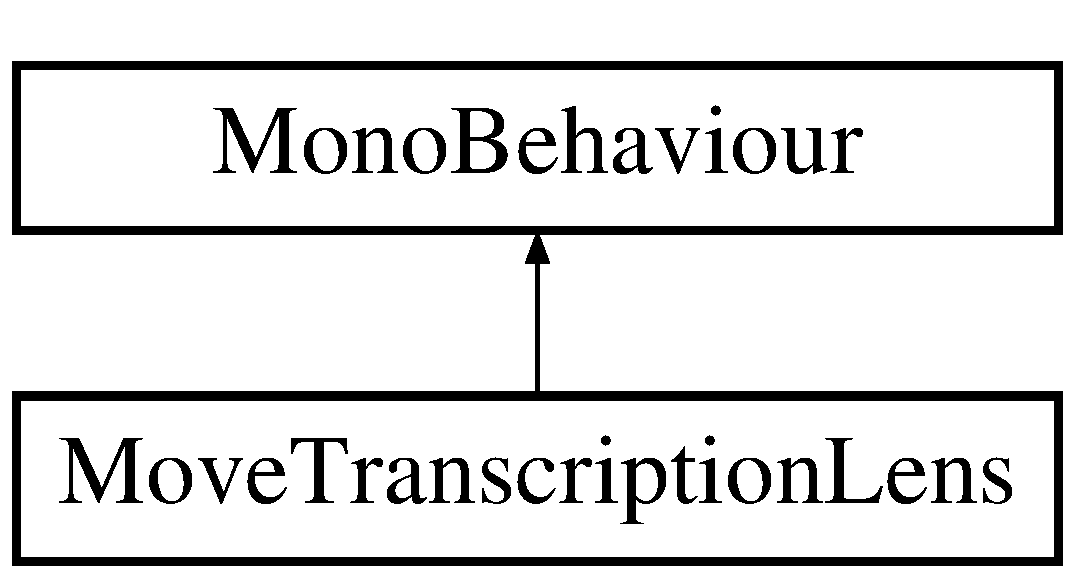
\includegraphics[height=2.000000cm]{class_move_transcription_lens}
\end{center}
\end{figure}
\subsection*{Public Attributes}
\begin{DoxyCompactItemize}
\item 
Image {\bf lens\+Img}
\begin{DoxyCompactList}\small\item\em The image of the lens. \end{DoxyCompactList}\item 
Image {\bf mask\+Img}
\begin{DoxyCompactList}\small\item\em The image of the mask. \end{DoxyCompactList}\end{DoxyCompactItemize}


\subsection{Detailed Description}
The transcription lens movement logic. 



\subsection{Member Data Documentation}
\index{Move\+Transcription\+Lens@{Move\+Transcription\+Lens}!lens\+Img@{lens\+Img}}
\index{lens\+Img@{lens\+Img}!Move\+Transcription\+Lens@{Move\+Transcription\+Lens}}
\subsubsection[{lens\+Img}]{\setlength{\rightskip}{0pt plus 5cm}Image Move\+Transcription\+Lens.\+lens\+Img}\label{class_move_transcription_lens_a5866efc3b483fb9ffe6143687db88718}


The image of the lens. 

\index{Move\+Transcription\+Lens@{Move\+Transcription\+Lens}!mask\+Img@{mask\+Img}}
\index{mask\+Img@{mask\+Img}!Move\+Transcription\+Lens@{Move\+Transcription\+Lens}}
\subsubsection[{mask\+Img}]{\setlength{\rightskip}{0pt plus 5cm}Image Move\+Transcription\+Lens.\+mask\+Img}\label{class_move_transcription_lens_aa6cfdf5315d72486178bc311132e8363}


The image of the mask. 



The documentation for this class was generated from the following file\+:\begin{DoxyCompactItemize}
\item 
Move\+Transcription\+Lens.\+cs\end{DoxyCompactItemize}

\section{Page\+Images Class Reference}
\label{class_page_images}\index{Page\+Images@{Page\+Images}}


Presents the I\+I\+IF images from a manifest on 6 pages.  


Inheritance diagram for Page\+Images\+:\begin{figure}[H]
\begin{center}
\leavevmode
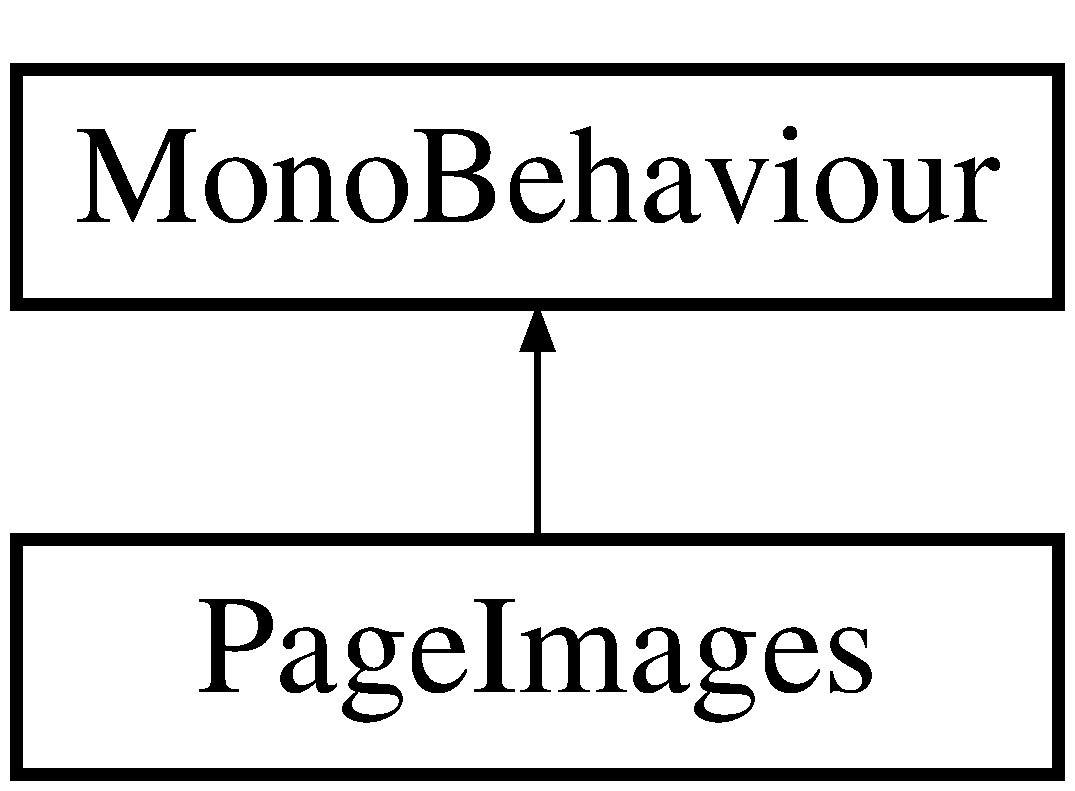
\includegraphics[height=2.000000cm]{class_page_images}
\end{center}
\end{figure}
\subsection*{Public Member Functions}
\begin{DoxyCompactItemize}
\item 
I\+Enumerator {\bf Turn\+Page\+Left} ()
\begin{DoxyCompactList}\small\item\em Shifts page\textquotesingle{}s textures to the left and loads the next two pages. \end{DoxyCompactList}\item 
I\+Enumerator {\bf Turn\+Page\+Right} ()
\begin{DoxyCompactList}\small\item\em Shifts page\textquotesingle{}s textures to the right and loads the previous two pages. \end{DoxyCompactList}\item 
bool {\bf Is\+Loading\+Left} ()
\begin{DoxyCompactList}\small\item\em Determines whether this instance is loading left pages. \end{DoxyCompactList}\item 
bool {\bf Is\+Loading\+Right} ()
\begin{DoxyCompactList}\small\item\em Determines whether this instance is loading right pages. \end{DoxyCompactList}\item 
void {\bf Show\+Annotations} (bool is\+Showing)
\begin{DoxyCompactList}\small\item\em Shows/\+Hides the annotations. \end{DoxyCompactList}\item 
void {\bf Update\+Annotations} ()
\begin{DoxyCompactList}\small\item\em Updates the annotations that are being drawn. \end{DoxyCompactList}\item 
{\bf Annotation.\+Annotation\+Box}[$\,$] {\bf Get\+Annotations} (int which)
\begin{DoxyCompactList}\small\item\em Gets the annotations for a specified page. \end{DoxyCompactList}\end{DoxyCompactItemize}
\subsection*{Public Attributes}
\begin{DoxyCompactItemize}
\item 
Renderer[$\,$] {\bf pages}
\begin{DoxyCompactList}\small\item\em The pages to present the I\+I\+IF images on. \end{DoxyCompactList}\item 
{\bf I\+I\+I\+F\+Image\+Get} {\bf iiif\+Image}
\begin{DoxyCompactList}\small\item\em Used to obtain the images. \end{DoxyCompactList}\item 
string {\bf manifest\+U\+RL}
\begin{DoxyCompactList}\small\item\em The manifest U\+RL. \end{DoxyCompactList}\item 
Texture2D {\bf loading\+Texture}
\begin{DoxyCompactList}\small\item\em The texture to display when loading images \end{DoxyCompactList}\item 
{\bf Annotation}[$\,$] {\bf annotation}
\begin{DoxyCompactList}\small\item\em Retrieve infomation about annotations on the pages. \end{DoxyCompactList}\item 
{\bf Annotation\+Drawer}[$\,$] {\bf drawers}
\begin{DoxyCompactList}\small\item\em The annotation drawers. \end{DoxyCompactList}\item 
{\bf Transcription\+Tool} {\bf left\+Trans}
\begin{DoxyCompactList}\small\item\em The left transcription. \end{DoxyCompactList}\item 
{\bf Transcription\+Tool} {\bf right\+Trans}
\begin{DoxyCompactList}\small\item\em The right transcription. \end{DoxyCompactList}\item 
Text {\bf page\+Display}
\begin{DoxyCompactList}\small\item\em The text that display the page number. \end{DoxyCompactList}\end{DoxyCompactItemize}


\subsection{Detailed Description}
Presents the I\+I\+IF images from a manifest on 6 pages. 



\subsection{Member Function Documentation}
\index{Page\+Images@{Page\+Images}!Get\+Annotations@{Get\+Annotations}}
\index{Get\+Annotations@{Get\+Annotations}!Page\+Images@{Page\+Images}}
\subsubsection[{Get\+Annotations(int which)}]{\setlength{\rightskip}{0pt plus 5cm}{\bf Annotation.\+Annotation\+Box} [$\,$] Page\+Images.\+Get\+Annotations (
\begin{DoxyParamCaption}
\item[{int}]{which}
\end{DoxyParamCaption}
)}\label{class_page_images_af563e42dd7774f6ea7a51a9e5668ddc0}


Gets the annotations for a specified page. 

\begin{DoxyReturn}{Returns}
The annotations for the page.
\end{DoxyReturn}

\begin{DoxyParams}{Parameters}
{\em which} & Which page to get the annotations for (0 for left, 1 for right).\\
\hline
\end{DoxyParams}
\index{Page\+Images@{Page\+Images}!Is\+Loading\+Left@{Is\+Loading\+Left}}
\index{Is\+Loading\+Left@{Is\+Loading\+Left}!Page\+Images@{Page\+Images}}
\subsubsection[{Is\+Loading\+Left()}]{\setlength{\rightskip}{0pt plus 5cm}bool Page\+Images.\+Is\+Loading\+Left (
\begin{DoxyParamCaption}
{}
\end{DoxyParamCaption}
)}\label{class_page_images_a5412e1d64104e009ad3cf9fa3c3351dd}


Determines whether this instance is loading left pages. 

\begin{DoxyReturn}{Returns}
{\ttfamily true} if this instance is loading left pages; otherwise, {\ttfamily false}.
\end{DoxyReturn}
\index{Page\+Images@{Page\+Images}!Is\+Loading\+Right@{Is\+Loading\+Right}}
\index{Is\+Loading\+Right@{Is\+Loading\+Right}!Page\+Images@{Page\+Images}}
\subsubsection[{Is\+Loading\+Right()}]{\setlength{\rightskip}{0pt plus 5cm}bool Page\+Images.\+Is\+Loading\+Right (
\begin{DoxyParamCaption}
{}
\end{DoxyParamCaption}
)}\label{class_page_images_a7fcf05646abee094ae39cdf725489414}


Determines whether this instance is loading right pages. 

\begin{DoxyReturn}{Returns}
{\ttfamily true} if this instance is loading right pages; otherwise, {\ttfamily false}.
\end{DoxyReturn}
\index{Page\+Images@{Page\+Images}!Show\+Annotations@{Show\+Annotations}}
\index{Show\+Annotations@{Show\+Annotations}!Page\+Images@{Page\+Images}}
\subsubsection[{Show\+Annotations(bool is\+Showing)}]{\setlength{\rightskip}{0pt plus 5cm}void Page\+Images.\+Show\+Annotations (
\begin{DoxyParamCaption}
\item[{bool}]{is\+Showing}
\end{DoxyParamCaption}
)}\label{class_page_images_aaaebf078a3aaff99a47b5ddbdbbd9dd7}


Shows/\+Hides the annotations. 


\begin{DoxyParams}{Parameters}
{\em is\+Showing} & If set to {\ttfamily true} shows annotations. Otherwise, hides annotations.\\
\hline
\end{DoxyParams}
\index{Page\+Images@{Page\+Images}!Turn\+Page\+Left@{Turn\+Page\+Left}}
\index{Turn\+Page\+Left@{Turn\+Page\+Left}!Page\+Images@{Page\+Images}}
\subsubsection[{Turn\+Page\+Left()}]{\setlength{\rightskip}{0pt plus 5cm}I\+Enumerator Page\+Images.\+Turn\+Page\+Left (
\begin{DoxyParamCaption}
{}
\end{DoxyParamCaption}
)}\label{class_page_images_a2d94ed5b60c041dd4550f4dfbca0ef94}


Shifts page\textquotesingle{}s textures to the left and loads the next two pages. 

\index{Page\+Images@{Page\+Images}!Turn\+Page\+Right@{Turn\+Page\+Right}}
\index{Turn\+Page\+Right@{Turn\+Page\+Right}!Page\+Images@{Page\+Images}}
\subsubsection[{Turn\+Page\+Right()}]{\setlength{\rightskip}{0pt plus 5cm}I\+Enumerator Page\+Images.\+Turn\+Page\+Right (
\begin{DoxyParamCaption}
{}
\end{DoxyParamCaption}
)}\label{class_page_images_a290f753eca727781c135ce41e6fcd48a}


Shifts page\textquotesingle{}s textures to the right and loads the previous two pages. 

\index{Page\+Images@{Page\+Images}!Update\+Annotations@{Update\+Annotations}}
\index{Update\+Annotations@{Update\+Annotations}!Page\+Images@{Page\+Images}}
\subsubsection[{Update\+Annotations()}]{\setlength{\rightskip}{0pt plus 5cm}void Page\+Images.\+Update\+Annotations (
\begin{DoxyParamCaption}
{}
\end{DoxyParamCaption}
)}\label{class_page_images_ad9678501582f1cb45563e2b294d97ced}


Updates the annotations that are being drawn. 



\subsection{Member Data Documentation}
\index{Page\+Images@{Page\+Images}!annotation@{annotation}}
\index{annotation@{annotation}!Page\+Images@{Page\+Images}}
\subsubsection[{annotation}]{\setlength{\rightskip}{0pt plus 5cm}{\bf Annotation} [$\,$] Page\+Images.\+annotation}\label{class_page_images_a6579d6330bcfb9f7b7782c84f39e8431}


Retrieve infomation about annotations on the pages. 

\index{Page\+Images@{Page\+Images}!drawers@{drawers}}
\index{drawers@{drawers}!Page\+Images@{Page\+Images}}
\subsubsection[{drawers}]{\setlength{\rightskip}{0pt plus 5cm}{\bf Annotation\+Drawer} [$\,$] Page\+Images.\+drawers}\label{class_page_images_a5113b509fe82ac0eb3670856860fa113}


The annotation drawers. 

\index{Page\+Images@{Page\+Images}!iiif\+Image@{iiif\+Image}}
\index{iiif\+Image@{iiif\+Image}!Page\+Images@{Page\+Images}}
\subsubsection[{iiif\+Image}]{\setlength{\rightskip}{0pt plus 5cm}{\bf I\+I\+I\+F\+Image\+Get} Page\+Images.\+iiif\+Image}\label{class_page_images_ac5c26cd4b70e28c0c13f18d6a0cc5b71}


Used to obtain the images. 

\index{Page\+Images@{Page\+Images}!left\+Trans@{left\+Trans}}
\index{left\+Trans@{left\+Trans}!Page\+Images@{Page\+Images}}
\subsubsection[{left\+Trans}]{\setlength{\rightskip}{0pt plus 5cm}{\bf Transcription\+Tool} Page\+Images.\+left\+Trans}\label{class_page_images_a640a7d43b34e9f47a2ade8c83c239c78}


The left transcription. 

\index{Page\+Images@{Page\+Images}!loading\+Texture@{loading\+Texture}}
\index{loading\+Texture@{loading\+Texture}!Page\+Images@{Page\+Images}}
\subsubsection[{loading\+Texture}]{\setlength{\rightskip}{0pt plus 5cm}Texture2D Page\+Images.\+loading\+Texture}\label{class_page_images_a23ff461069def11e8c328474c28a6516}


The texture to display when loading images 

\index{Page\+Images@{Page\+Images}!manifest\+U\+RL@{manifest\+U\+RL}}
\index{manifest\+U\+RL@{manifest\+U\+RL}!Page\+Images@{Page\+Images}}
\subsubsection[{manifest\+U\+RL}]{\setlength{\rightskip}{0pt plus 5cm}string Page\+Images.\+manifest\+U\+RL}\label{class_page_images_a4392dd9e57f3dc4f97a90c9deea5fa50}


The manifest U\+RL. 

\index{Page\+Images@{Page\+Images}!page\+Display@{page\+Display}}
\index{page\+Display@{page\+Display}!Page\+Images@{Page\+Images}}
\subsubsection[{page\+Display}]{\setlength{\rightskip}{0pt plus 5cm}Text Page\+Images.\+page\+Display}\label{class_page_images_ae0dfe0e7e9f87ff9f0724cfdf856eea0}


The text that display the page number. 

\index{Page\+Images@{Page\+Images}!pages@{pages}}
\index{pages@{pages}!Page\+Images@{Page\+Images}}
\subsubsection[{pages}]{\setlength{\rightskip}{0pt plus 5cm}Renderer [$\,$] Page\+Images.\+pages}\label{class_page_images_ab33e023afe9968299aee2c600a9b6670}


The pages to present the I\+I\+IF images on. 

\index{Page\+Images@{Page\+Images}!right\+Trans@{right\+Trans}}
\index{right\+Trans@{right\+Trans}!Page\+Images@{Page\+Images}}
\subsubsection[{right\+Trans}]{\setlength{\rightskip}{0pt plus 5cm}{\bf Transcription\+Tool} Page\+Images.\+right\+Trans}\label{class_page_images_a43dd571101b0554c29a48c8fab263042}


The right transcription. 



The documentation for this class was generated from the following file\+:\begin{DoxyCompactItemize}
\item 
Page\+Images.\+cs\end{DoxyCompactItemize}

\section{Pop\+Up\+Box Class Reference}
\label{class_pop_up_box}\index{Pop\+Up\+Box@{Pop\+Up\+Box}}


A popup box used to get input from the user.  


Inheritance diagram for Pop\+Up\+Box\+:\begin{figure}[H]
\begin{center}
\leavevmode
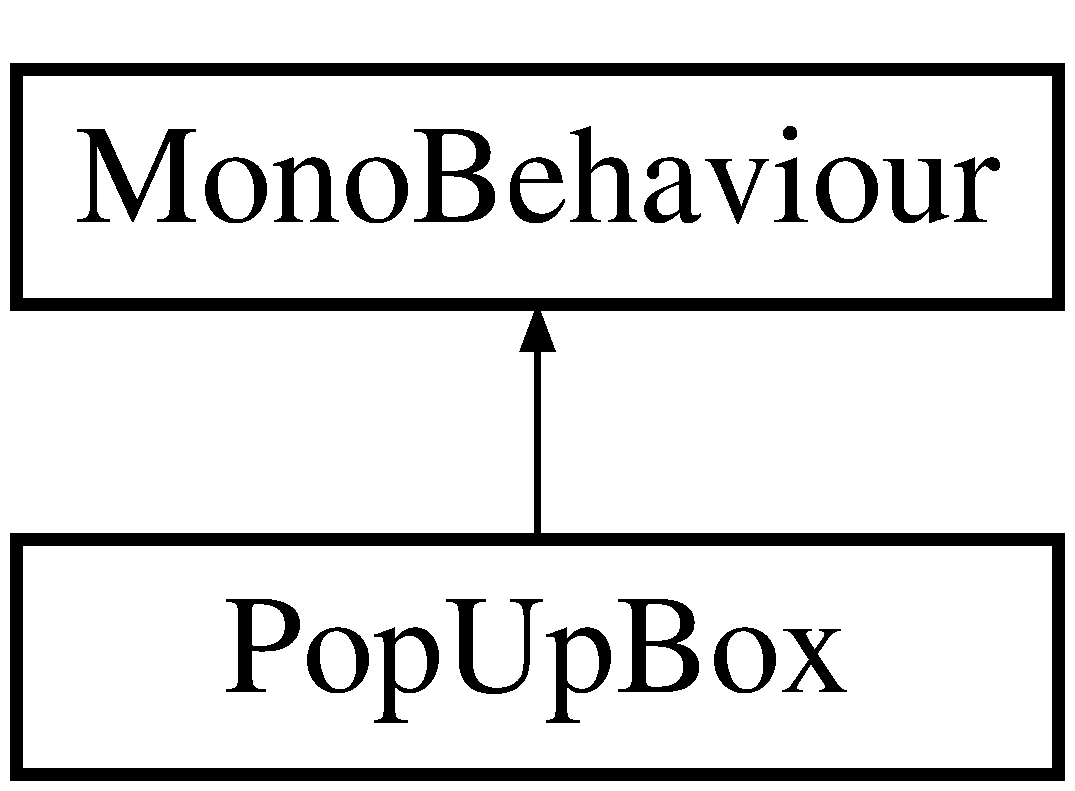
\includegraphics[height=2.000000cm]{class_pop_up_box}
\end{center}
\end{figure}
\subsection*{Public Member Functions}
\begin{DoxyCompactItemize}
\item 
I\+Enumerator {\bf Pop\+Up} ()
\begin{DoxyCompactList}\small\item\em Display the popup window. \end{DoxyCompactList}\item 
string {\bf get\+Text} ()
\begin{DoxyCompactList}\small\item\em Gets the text inputed by the user. \end{DoxyCompactList}\item 
void {\bf Submit} ()
\begin{DoxyCompactList}\small\item\em The action to perform when the user submits their input. \end{DoxyCompactList}\item 
void {\bf Cancel} ()
\begin{DoxyCompactList}\small\item\em The action to perform when the user cancels their input. \end{DoxyCompactList}\item 
void {\bf reset} ()
\begin{DoxyCompactList}\small\item\em Reset this instance. \end{DoxyCompactList}\end{DoxyCompactItemize}
\subsection*{Public Attributes}
\begin{DoxyCompactItemize}
\item 
Input\+Field {\bf input}
\begin{DoxyCompactList}\small\item\em The input field to get input from. \end{DoxyCompactList}\end{DoxyCompactItemize}


\subsection{Detailed Description}
A popup box used to get input from the user. 



\subsection{Member Function Documentation}
\index{Pop\+Up\+Box@{Pop\+Up\+Box}!Cancel@{Cancel}}
\index{Cancel@{Cancel}!Pop\+Up\+Box@{Pop\+Up\+Box}}
\subsubsection[{Cancel()}]{\setlength{\rightskip}{0pt plus 5cm}void Pop\+Up\+Box.\+Cancel (
\begin{DoxyParamCaption}
{}
\end{DoxyParamCaption}
)}\label{class_pop_up_box_af40a3029d3e07286c29b859181072ee8}


The action to perform when the user cancels their input. 

\index{Pop\+Up\+Box@{Pop\+Up\+Box}!get\+Text@{get\+Text}}
\index{get\+Text@{get\+Text}!Pop\+Up\+Box@{Pop\+Up\+Box}}
\subsubsection[{get\+Text()}]{\setlength{\rightskip}{0pt plus 5cm}string Pop\+Up\+Box.\+get\+Text (
\begin{DoxyParamCaption}
{}
\end{DoxyParamCaption}
)}\label{class_pop_up_box_ac80e75be1581aeacb6727bac277b5e1c}


Gets the text inputed by the user. 

\begin{DoxyReturn}{Returns}
The text inputed by the user.
\end{DoxyReturn}
\index{Pop\+Up\+Box@{Pop\+Up\+Box}!Pop\+Up@{Pop\+Up}}
\index{Pop\+Up@{Pop\+Up}!Pop\+Up\+Box@{Pop\+Up\+Box}}
\subsubsection[{Pop\+Up()}]{\setlength{\rightskip}{0pt plus 5cm}I\+Enumerator Pop\+Up\+Box.\+Pop\+Up (
\begin{DoxyParamCaption}
{}
\end{DoxyParamCaption}
)}\label{class_pop_up_box_a29566d075e78858a091f201798e49555}


Display the popup window. 

\index{Pop\+Up\+Box@{Pop\+Up\+Box}!reset@{reset}}
\index{reset@{reset}!Pop\+Up\+Box@{Pop\+Up\+Box}}
\subsubsection[{reset()}]{\setlength{\rightskip}{0pt plus 5cm}void Pop\+Up\+Box.\+reset (
\begin{DoxyParamCaption}
{}
\end{DoxyParamCaption}
)}\label{class_pop_up_box_acc42337540e97fd45d2f5e6ed8451a4c}


Reset this instance. 

\index{Pop\+Up\+Box@{Pop\+Up\+Box}!Submit@{Submit}}
\index{Submit@{Submit}!Pop\+Up\+Box@{Pop\+Up\+Box}}
\subsubsection[{Submit()}]{\setlength{\rightskip}{0pt plus 5cm}void Pop\+Up\+Box.\+Submit (
\begin{DoxyParamCaption}
{}
\end{DoxyParamCaption}
)}\label{class_pop_up_box_abdc32668e20f43015bc213473fb9412a}


The action to perform when the user submits their input. 



\subsection{Member Data Documentation}
\index{Pop\+Up\+Box@{Pop\+Up\+Box}!input@{input}}
\index{input@{input}!Pop\+Up\+Box@{Pop\+Up\+Box}}
\subsubsection[{input}]{\setlength{\rightskip}{0pt plus 5cm}Input\+Field Pop\+Up\+Box.\+input}\label{class_pop_up_box_a9012f3c4ec923daa534d57d011d2a0ef}


The input field to get input from. 



The documentation for this class was generated from the following file\+:\begin{DoxyCompactItemize}
\item 
Pop\+Up\+Box.\+cs\end{DoxyCompactItemize}

\section{Transcription\+Tool Class Reference}
\label{class_transcription_tool}\index{Transcription\+Tool@{Transcription\+Tool}}


Displays the transcription of the text.  


Inheritance diagram for Transcription\+Tool\+:\begin{figure}[H]
\begin{center}
\leavevmode
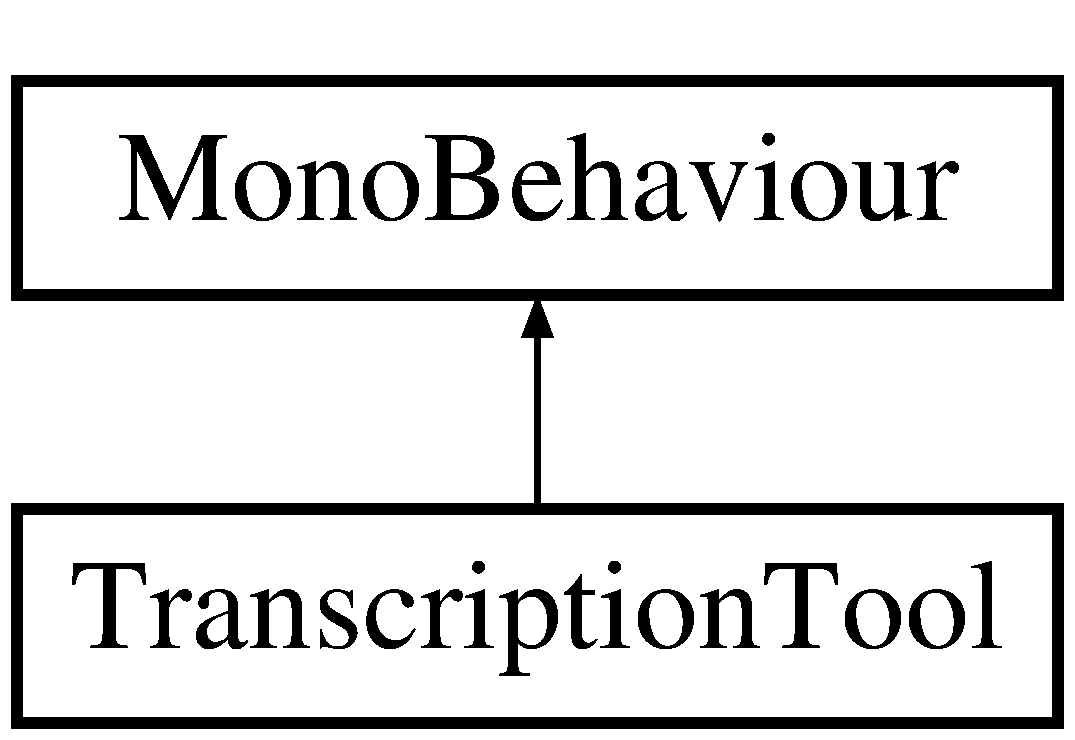
\includegraphics[height=2.000000cm]{class_transcription_tool}
\end{center}
\end{figure}
\subsection*{Public Member Functions}
\begin{DoxyCompactItemize}
\item 
void {\bf Updates\+Transcriptions} ({\bf Annotation.\+Annotation\+Box} annos)
\begin{DoxyCompactList}\small\item\em Updates the transcription. \end{DoxyCompactList}\end{DoxyCompactItemize}
\subsection*{Public Attributes}
\begin{DoxyCompactItemize}
\item 
Transform {\bf top\+Left}
\begin{DoxyCompactList}\small\item\em The location of the top left corner of the page. \end{DoxyCompactList}\item 
Transform {\bf bottom\+Right}
\begin{DoxyCompactList}\small\item\em The location of the bottom right corner of the page. \end{DoxyCompactList}\item 
Rect\+Transform {\bf annotations}
\begin{DoxyCompactList}\small\item\em The boundaries of the transcription. \end{DoxyCompactList}\item 
Transform {\bf canvas}
\begin{DoxyCompactList}\small\item\em The canvas. \end{DoxyCompactList}\end{DoxyCompactItemize}


\subsection{Detailed Description}
Displays the transcription of the text. 



\subsection{Member Function Documentation}
\index{Transcription\+Tool@{Transcription\+Tool}!Updates\+Transcriptions@{Updates\+Transcriptions}}
\index{Updates\+Transcriptions@{Updates\+Transcriptions}!Transcription\+Tool@{Transcription\+Tool}}
\subsubsection[{Updates\+Transcriptions(\+Annotation.\+Annotation\+Box annos)}]{\setlength{\rightskip}{0pt plus 5cm}void Transcription\+Tool.\+Updates\+Transcriptions (
\begin{DoxyParamCaption}
\item[{{\bf Annotation.\+Annotation\+Box}}]{annos}
\end{DoxyParamCaption}
)}\label{class_transcription_tool_a524c1bac32c7492e41bf7d36678da8ca}


Updates the transcription. 


\begin{DoxyParams}{Parameters}
{\em annos} & The new transcription.\\
\hline
\end{DoxyParams}


\subsection{Member Data Documentation}
\index{Transcription\+Tool@{Transcription\+Tool}!annotations@{annotations}}
\index{annotations@{annotations}!Transcription\+Tool@{Transcription\+Tool}}
\subsubsection[{annotations}]{\setlength{\rightskip}{0pt plus 5cm}Rect\+Transform Transcription\+Tool.\+annotations}\label{class_transcription_tool_a0f13c7a0e9de49ce6d51c1d7e27cab17}


The boundaries of the transcription. 

\index{Transcription\+Tool@{Transcription\+Tool}!bottom\+Right@{bottom\+Right}}
\index{bottom\+Right@{bottom\+Right}!Transcription\+Tool@{Transcription\+Tool}}
\subsubsection[{bottom\+Right}]{\setlength{\rightskip}{0pt plus 5cm}Transform Transcription\+Tool.\+bottom\+Right}\label{class_transcription_tool_a7fc3f48e81e40135739550028b5ee63b}


The location of the bottom right corner of the page. 

\index{Transcription\+Tool@{Transcription\+Tool}!canvas@{canvas}}
\index{canvas@{canvas}!Transcription\+Tool@{Transcription\+Tool}}
\subsubsection[{canvas}]{\setlength{\rightskip}{0pt plus 5cm}Transform Transcription\+Tool.\+canvas}\label{class_transcription_tool_a1a5a59f37fde0ed8d52fa2af9d7a3561}


The canvas. 

\index{Transcription\+Tool@{Transcription\+Tool}!top\+Left@{top\+Left}}
\index{top\+Left@{top\+Left}!Transcription\+Tool@{Transcription\+Tool}}
\subsubsection[{top\+Left}]{\setlength{\rightskip}{0pt plus 5cm}Transform Transcription\+Tool.\+top\+Left}\label{class_transcription_tool_ac5ef003ae5d7745a53d8ee5fbb3ffda2}


The location of the top left corner of the page. 



The documentation for this class was generated from the following file\+:\begin{DoxyCompactItemize}
\item 
Transcription\+Tool.\+cs\end{DoxyCompactItemize}

\section{U\+I\+Pop\+Up Class Reference}
\label{class_u_i_pop_up}\index{U\+I\+Pop\+Up@{U\+I\+Pop\+Up}}


Hides/\+Shows UI elements.  


Inheritance diagram for U\+I\+Pop\+Up\+:\begin{figure}[H]
\begin{center}
\leavevmode
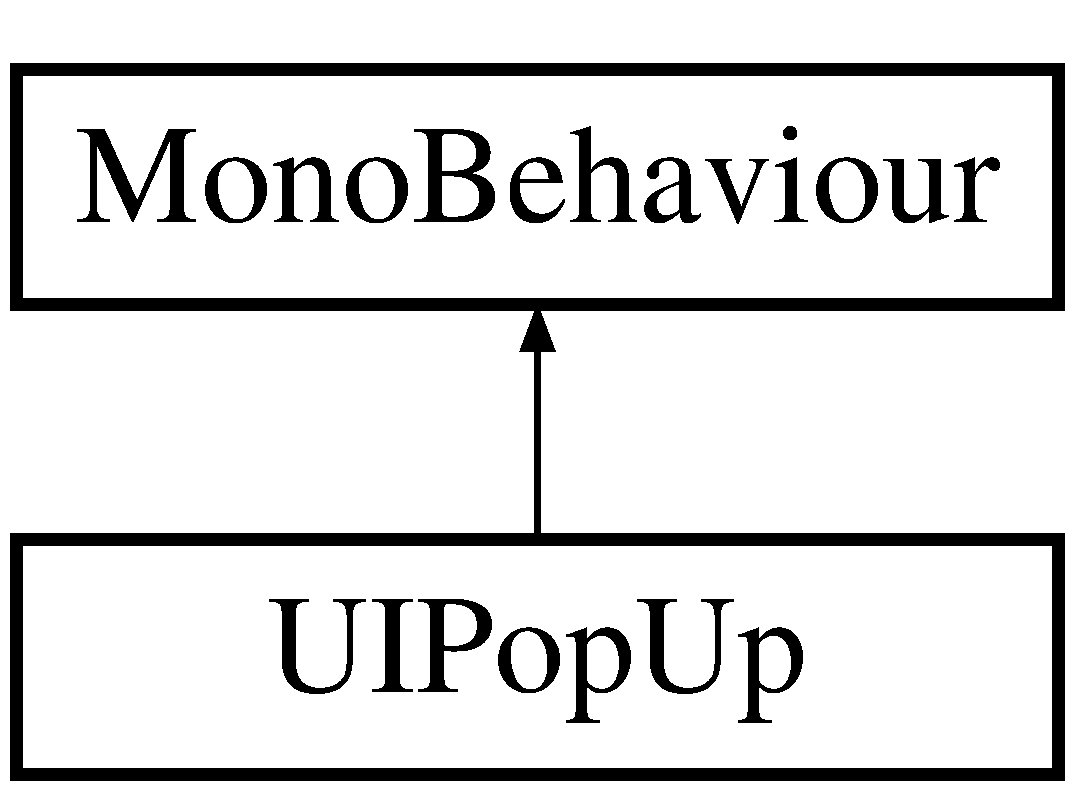
\includegraphics[height=2.000000cm]{class_u_i_pop_up}
\end{center}
\end{figure}
\subsection*{Public Member Functions}
\begin{DoxyCompactItemize}
\item 
bool {\bf Is\+Showing} ()
\begin{DoxyCompactList}\small\item\em Determines whether this instance is showing. \end{DoxyCompactList}\end{DoxyCompactItemize}
\subsection*{Public Attributes}
\begin{DoxyCompactItemize}
\item 
float {\bf hideY}
\begin{DoxyCompactList}\small\item\em The vertical position the UI should move to for hiding. \end{DoxyCompactList}\item 
float {\bf showY}
\begin{DoxyCompactList}\small\item\em The vertical position the UI should move to for showing. \end{DoxyCompactList}\item 
float {\bf trigger\+Pos}
\begin{DoxyCompactList}\small\item\em How low/high the cursor needs to be to show the UI (0.\+0f for bottom of the screen, 1.\+0f for top of the screen). \end{DoxyCompactList}\item 
Rect\+Transform {\bf pos}
\begin{DoxyCompactList}\small\item\em The position of the UI. \end{DoxyCompactList}\item 
bool {\bf hide\+Above}
\begin{DoxyCompactList}\small\item\em Shoud the UI hide from the top of the screen, or the bottom? \end{DoxyCompactList}\end{DoxyCompactItemize}


\subsection{Detailed Description}
Hides/\+Shows UI elements. 



\subsection{Member Function Documentation}
\index{U\+I\+Pop\+Up@{U\+I\+Pop\+Up}!Is\+Showing@{Is\+Showing}}
\index{Is\+Showing@{Is\+Showing}!U\+I\+Pop\+Up@{U\+I\+Pop\+Up}}
\subsubsection[{Is\+Showing()}]{\setlength{\rightskip}{0pt plus 5cm}bool U\+I\+Pop\+Up.\+Is\+Showing (
\begin{DoxyParamCaption}
{}
\end{DoxyParamCaption}
)}\label{class_u_i_pop_up_a71354e6d0c5b79a2af374164a3e07036}


Determines whether this instance is showing. 

\begin{DoxyReturn}{Returns}
{\ttfamily true} if this instance is showing; otherwise, {\ttfamily false}.
\end{DoxyReturn}


\subsection{Member Data Documentation}
\index{U\+I\+Pop\+Up@{U\+I\+Pop\+Up}!hide\+Above@{hide\+Above}}
\index{hide\+Above@{hide\+Above}!U\+I\+Pop\+Up@{U\+I\+Pop\+Up}}
\subsubsection[{hide\+Above}]{\setlength{\rightskip}{0pt plus 5cm}bool U\+I\+Pop\+Up.\+hide\+Above}\label{class_u_i_pop_up_a08dd327672fa2988751468c64624b49c}


Shoud the UI hide from the top of the screen, or the bottom? 

\index{U\+I\+Pop\+Up@{U\+I\+Pop\+Up}!hideY@{hideY}}
\index{hideY@{hideY}!U\+I\+Pop\+Up@{U\+I\+Pop\+Up}}
\subsubsection[{hideY}]{\setlength{\rightskip}{0pt plus 5cm}float U\+I\+Pop\+Up.\+hideY}\label{class_u_i_pop_up_af348533bd87896b58b9b71a63cbbddba}


The vertical position the UI should move to for hiding. 

\index{U\+I\+Pop\+Up@{U\+I\+Pop\+Up}!pos@{pos}}
\index{pos@{pos}!U\+I\+Pop\+Up@{U\+I\+Pop\+Up}}
\subsubsection[{pos}]{\setlength{\rightskip}{0pt plus 5cm}Rect\+Transform U\+I\+Pop\+Up.\+pos}\label{class_u_i_pop_up_afd353b97181fa8fbad1222f0af69d1d2}


The position of the UI. 

\index{U\+I\+Pop\+Up@{U\+I\+Pop\+Up}!showY@{showY}}
\index{showY@{showY}!U\+I\+Pop\+Up@{U\+I\+Pop\+Up}}
\subsubsection[{showY}]{\setlength{\rightskip}{0pt plus 5cm}float U\+I\+Pop\+Up.\+showY}\label{class_u_i_pop_up_a4bd553bffe09e1bcf5c08f1bc30d7ea0}


The vertical position the UI should move to for showing. 

\index{U\+I\+Pop\+Up@{U\+I\+Pop\+Up}!trigger\+Pos@{trigger\+Pos}}
\index{trigger\+Pos@{trigger\+Pos}!U\+I\+Pop\+Up@{U\+I\+Pop\+Up}}
\subsubsection[{trigger\+Pos}]{\setlength{\rightskip}{0pt plus 5cm}float U\+I\+Pop\+Up.\+trigger\+Pos}\label{class_u_i_pop_up_adfe9128f5953b521ac2730d8092eb66d}


How low/high the cursor needs to be to show the UI (0.\+0f for bottom of the screen, 1.\+0f for top of the screen). 



The documentation for this class was generated from the following file\+:\begin{DoxyCompactItemize}
\item 
U\+I\+Pop\+Up.\+cs\end{DoxyCompactItemize}

%--- End generated contents ---

% Index
\backmatter
\newpage
\phantomsection
\clearemptydoublepage
\addcontentsline{toc}{chapter}{Index}
\printindex

\end{document}
